% Options for packages loaded elsewhere
\PassOptionsToPackage{unicode}{hyperref}
\PassOptionsToPackage{hyphens}{url}
\documentclass[
]{book}
\usepackage{xcolor}
\usepackage{amsmath,amssymb}
\setcounter{secnumdepth}{-\maxdimen} % remove section numbering
\usepackage{iftex}
\ifPDFTeX
  \usepackage[T1]{fontenc}
  \usepackage[utf8]{inputenc}
  \usepackage{textcomp} % provide euro and other symbols
\else % if luatex or xetex
  \usepackage{unicode-math} % this also loads fontspec
  \defaultfontfeatures{Scale=MatchLowercase}
  \defaultfontfeatures[\rmfamily]{Ligatures=TeX,Scale=1}
\fi
\usepackage{lmodern}
\ifPDFTeX\else
  % xetex/luatex font selection
\fi
% Use upquote if available, for straight quotes in verbatim environments
\IfFileExists{upquote.sty}{\usepackage{upquote}}{}
\IfFileExists{microtype.sty}{% use microtype if available
  \usepackage[]{microtype}
  \UseMicrotypeSet[protrusion]{basicmath} % disable protrusion for tt fonts
}{}
\makeatletter
\@ifundefined{KOMAClassName}{% if non-KOMA class
  \IfFileExists{parskip.sty}{%
    \usepackage{parskip}
  }{% else
    \setlength{\parindent}{0pt}
    \setlength{\parskip}{6pt plus 2pt minus 1pt}}
}{% if KOMA class
  \KOMAoptions{parskip=half}}
\makeatother
\usepackage{graphicx}
\makeatletter
\newsavebox\pandoc@box
\newcommand*\pandocbounded[1]{% scales image to fit in text height/width
  \sbox\pandoc@box{#1}%
  \Gscale@div\@tempa{\textheight}{\dimexpr\ht\pandoc@box+\dp\pandoc@box\relax}%
  \Gscale@div\@tempb{\linewidth}{\wd\pandoc@box}%
  \ifdim\@tempb\p@<\@tempa\p@\let\@tempa\@tempb\fi% select the smaller of both
  \ifdim\@tempa\p@<\p@\scalebox{\@tempa}{\usebox\pandoc@box}%
  \else\usebox{\pandoc@box}%
  \fi%
}
% Set default figure placement to htbp
\def\fps@figure{htbp}
\makeatother
\setlength{\emergencystretch}{3em} % prevent overfull lines
\providecommand{\tightlist}{%
  \setlength{\itemsep}{0pt}\setlength{\parskip}{0pt}}
\usepackage{bookmark}
\IfFileExists{xurl.sty}{\usepackage{xurl}}{} % add URL line breaks if available
\urlstyle{same}
\hypersetup{
  hidelinks,
  pdfcreator={LaTeX via pandoc}}

\author{}
\date{}

\begin{document}
\frontmatter

\mainmatter
\chapter{EMT untuk Perhitungan Aljabar}\label{emt-untuk-perhitungan-aljabar}

Pada notebook ini Anda belajar menggunakan EMT untuk melakukan berbagai perhitungan terkait dengan materi atau topik dalam Aljabar. Kegiatan yang harus Anda lakukan adalah sebagai berikut:

\begin{itemize}
\item
  Membaca secara cermat dan teliti notebook ini;
\item
  Menerjemahkan teks bahasa Inggris ke bahasa Indonesia;
\item
  Mencoba contoh-contoh perhitungan (perintah EMT) dengan cara
\item
  meng-ENTER setiap perintah EMT yang ada (pindahkan kursor ke baris
\item
  perintah)
\item
  Jika perlu Anda dapat memodifikasi perintah yang ada dan memberikan
\item
  keterangan/penjelasan tambahan terkait hasilnya.
\item
  Menyisipkan baris-baris perintah baru untuk mengerjakan soal-soal
\item
  Aljabar dari file PDF yang saya berikan;
\item
  Memberi catatan hasilnya.
\item
  Jika perlu tuliskan soalnya pada teks notebook (menggunakan format
\item
  LaTeX).
\item
  Gunakan tampilan hasil semua perhitungan yang eksak atau simbolik
\item
  dengan format LaTeX. (Seperti contoh-contoh pada notebook ini.)
\end{itemize}

\section{Contoh pertama}\label{contoh-pertama}

Menyederhanakan bentuk aljabar:

\[6x^{-3}y^5\times -7x^2y^{-9}\]\textgreater\$\&6*x\textsuperscript{(-3)*y}5*-7*x\textsuperscript{2*y}(-9)

\[-\frac{42}{x\,y^4}\]Menjabarkan:

\[(6x^{-3}+y^5)(-7x^2-y^{-9})\]\textgreater\$\&showev('expand((6*x\textsuperscript{(-3)+y}5)*(-7*x\textsuperscript{2-y}(-9))))

\[{\it expand}\left(\left(-\frac{1}{y^9}-7\,x^2\right)\,\left(y^5+  \frac{6}{x^3}\right)\right)=-7\,x^2\,y^5-\frac{1}{y^4}-\frac{6}{x^3  \,y^9}-\frac{42}{x}\]\#\# Contoh lainnya

\[(\frac {24a^{10}b^{-8}c^7}{12a^6b^{-3}c^5})^{-5}\]\textgreater\$\&((24*a\textsuperscript{(10)*b}(-8)*c\textsuperscript{(7))/(12*a}6*b\textsuperscript{(-3)*c}5))\^{}-5

\[\frac{b^{25}}{32\,a^{20}\,c^{10}}\]\[(\frac{125p^{12}q^{-14}r^{22}}{25p^8q^6r^{-15}})^{-4}\]\textgreater\$\&((125*p\textsuperscript{(12)*q}(-14)*r\textsuperscript{(22))/(25*p}6*q\textsuperscript{(6)*r}(-15)))\^{}-4

\[\frac{q^{80}}{625\,p^{24}\,r^{148}}\]\[(m^{x-b}\times n^{x+b})^x(m^bn^{-b})^x\]\textgreater\$\&(m\textsuperscript{(x-b)*n}(x+b))\textsuperscript{x*(m}b*n\textsuperscript{(-b))}x

\[\left(\frac{m^{b}}{n^{b}}\right)^{x}\,\left(m^{x-b}\,n^{x+b}\right)  ^{x}\]\[(-5m^4n^2)(6m^2n^3)\]\textgreater\$\&(-5*m\textsuperscript{4*n}2)*(6*m\textsuperscript{2*n}3)

\[-30\,m^6\,n^5\]\[(8y^5)(9y)\]\textgreater\$\&(8*y\^{}5)*(9*y)

\[72\,y^6\]\#\# Baris Perintah

Baris perintah Euler terdiri dari satu atau beberapa perintah Euler diikuti dengan titik koma ``;'' atau koma ``,''. Titik koma mencegah pencetakan hasilnya. Koma setelah perintah terakhir dapat dihilangkan.

Baris perintah berikut hanya akan mencetak hasil ekspresi, bukan tugas atau perintah format.

\textgreater r:=2; h:=4; pi*r\^{}2*h/3

\begin{verbatim}
16.7551608191
\end{verbatim}

Perintah harus dipisahkan dengan bagian kosong. Baris perintah berikut mencetak dua hasil.

\textgreater pi*2*r*h, \%+2*pi*r*h // Ingat tanda \% menyatakan hasil perhitungan terakhir sebelumnya

\begin{verbatim}
50.2654824574
100.530964915
\end{verbatim}

Baris perintah dijalankan sesuai urutan yang ditekan kembali oleh pengguna. Jadi, Anda mendapatkan nilai baru setiap kali Anda menjalankan baris yang kedua.

\textgreater x := 1;

\textgreater x := cos(x) // nilai cosinus (x dalam radian)

\begin{verbatim}
0.540302305868
\end{verbatim}

\textgreater x := cos(x)

\begin{verbatim}
0.857553215846
\end{verbatim}

Jika dua baris dihubungkan dengan ``\ldots{}'' kedua baris akan selalu dijalankan secara bersamaan.

\textgreater x := 1.5; \ldots{}\\
\textgreater{} x := (x+2/x)/2, x := (x+2/x)/2, x := (x+2/x)/2,

\begin{verbatim}
1.41666666667
1.41421568627
1.41421356237
\end{verbatim}

Ini juga merupakan cara yang baik untuk menyebarkan perintah panjang ke dua baris atau lebih. Anda dapat menekan Ctrl+Return untuk membagi baris menjadi dua pada posisi kursor saat ini, atau Ctrl+Back untuk menggabungkan baris.

Untuk melipat semua multi-garis tekan Ctrl+L. Maka baris-baris berikutnya hanya akan terlihat, jika salah satunya mendapat fokus. Untuk melipat satu multi-baris, mulailah baris pertama dengan ``\%+''.

\textgreater\%+ x=4+5; \ldots{}\\
\textgreater{} // Garis ini tidak akan terlihat setelah kursor keluar dari garis

Baris yang dimulai dengan \%\% tidak akan terlihat sama sekali.

\begin{verbatim}
81
\end{verbatim}

Euler mendukung loop (pengulangan) di baris perintah, asalkan cocok ke dalam satu baris atau multi-baris. Tentu saja, pembatasan ini tidak berlaku dalam program. Untuk informasi lebih lanjut lihat pendahuluan berikut.

\textgreater x=1; for i=1 to 5; x := (x+2/x)/2, end; // menghitung akar 2

\begin{verbatim}
1.5
1.41666666667
1.41421568627
1.41421356237
1.41421356237
\end{verbatim}

Tidak apa-apa menggunakan multi-baris. Pastikan baris diakhiri dengan ``\ldots{}''.

\textgreater x := 1.5; // komentar buka di sini sebelum \ldots{}\\
\textgreater{} repeat xnew:=(x+2/x)/2; until xnew\textasciitilde=x; \ldots{}\\
\textgreater{} x := xnew; \ldots{}\\
\textgreater{} end; \ldots{}\\
\textgreater{} x,

\begin{verbatim}
1.41421356237
\end{verbatim}

Struktur bersyarat juga berfungsi.

\textgreater if E\textsuperscript{pi\textgreater pi}E; then ``Thought so!'', endif;

\begin{verbatim}
Thought so!
\end{verbatim}

Saat Anda menjalankan perintah, kursor dapat berada di posisi mana pun di baris perintah. Anda dapat kembali ke perintah sebelumnya atau melompat ke perintah berikutnya dengan tombol panah. Atau Anda dapat mengklik bagian komentar di atas perintah untuk membuka perintah.

Saat Anda menggerakkan kursor di sepanjang baris, pasangan tanda kurung atau tanda kurung buka dan tutup akan disorot. Juga, perhatikan baris status. Setelah tanda kurung buka dari fungsi sqrt(), baris status akan menampilkan teks bantuan untuk fungsi tersebut. Jalankan perintah dengan kunci kembali.

\textgreater sqrt(sin(10°)/cos(20°))

\begin{verbatim}
0.429875017772
\end{verbatim}

Untuk melihat bantuan untuk perintah terbaru, buka jendela bantuan dengan F1. Di sana, Anda dapat memasukkan teks untuk dicari. Pada baris kosong, bantuan untuk jendela bantuan akan ditampilkan. Anda dapat menekan escape untuk menghapus baris, atau untuk menutup jendela bantuan.

Anda dapat mengklik dua kali pada perintah apa pun untuk membuka bantuan untuk perintah ini. Coba klik dua kali perintah exp di bawah ini pada baris perintah.

\textgreater exp(log(2.5))

\begin{verbatim}
2.5
\end{verbatim}

Anda juga dapat menyalin (copy) dan menempel (paste) di Euler. Gunakan Ctrl+C dan Ctrl+V untuk ini. Untuk menandai teks, seret mouse atau gunakan shift bersamaan dengan tombol kursor apa pun. Selain itu, Anda dapat menyalin tanda kurung yang disorot.

\section{Contoh lainnya}\label{contoh-lainnya}

\[cos(45) \]\textgreater cos(45°)

\begin{verbatim}
0.707106781187
\end{verbatim}

\[tan (85.4)\]\textgreater tan(85.4°)

\begin{verbatim}
12.4288310198
\end{verbatim}

\[\frac {pi}{4}\]\textgreater pi/4

\begin{verbatim}
0.785398163397
\end{verbatim}

\[\frac{3pi}{2}\]\textgreater3*pi/2

\begin{verbatim}
4.71238898038
\end{verbatim}

\[8pi=...radian\]\textgreater pi=22/7;

\textgreater8*pi

\begin{verbatim}
25.1428571429
\end{verbatim}

\section{Sintaks Dasar}\label{sintaks-dasar}

Euler mengetahui fungsi matematika yang biasa digunakan. Seperti yang Anda lihat di atas, fungsi trigonometri bekerja dalam radian atau derajat. Untuk mengonversi ke derajat, tambahkan simbol derajat (dengan tombol F7) ke nilainya, atau gunakan fungsi rad(x). Fungsi akar kuadrat disebut sqrt di Euler. Tentu saja, bisa juga menggunakan x\^{}(1/2).

Untuk menyetel variabel, gunakan ``='' atau ``:=''. Demi kejelasan, pendahuluan ini menggunakan bentuk yang terakhir. Spasi tidak penting. Tapi diharapkan ada jarak antar perintah.

Beberapa perintah dalam satu baris dipisahkan dengan ``,'' atau ``;''. Titik koma menekan keluaran perintah. Di akhir baris perintah, ``,'' diasumsikan, jika ``;'' hilang.

\textgreater g:=9.81; t:=2.5; 1/2*g*t\^{}2

\begin{verbatim}
30.65625
\end{verbatim}

EMT menggunakan sintaks pemrograman untuk ekspresi. Untuk memasukkan

\[e^2 \cdot \left( \frac{1}{3+4 \log(0.6)}+\frac{1}{7} \right)\]Anda harus mengatur tanda kurung yang benar dan menggunakan / untuk pecahan. Perhatikan tanda kurung yang disorot untuk mendapatkan bantuan. Perhatikan bahwa konstanta Euler e diberi nama E dalam EMT.

\textgreater E\^{}2*(1/(3+4*log(0.6))+1/7)

\begin{verbatim}
8.77908249441
\end{verbatim}

Untuk menghitung ekspresi rumit seperti

\[\left(\frac{\frac17 + \frac18 + 2}{\frac13 + \frac12}\right)^2 \pi\]Anda harus memasukkannya dalam form baris.

\textgreater((1/7 + 1/8 + 2) / (1/3 + 1/2))\^{}2 * pi

\begin{verbatim}
23.2671801626
\end{verbatim}

Letakkan tanda kurung dengan hati-hati di sekitar sub-ekspresi yang perlu dihitung terlebih dahulu. EMT membantu Anda dengan menyorot ekspresi yang mengakhiri tanda kurung tutup. Anda juga harus memasukkan nama ``pi'' untuk huruf Yunani pi.

Hasil perhitungan ini berupa bilangan floating point. Ini secara default dicetak dengan akurasi sekitar 12 digit. Di baris perintah berikut, kita juga mempelajari bagaimana kita bisa merujuk ke hasil sebelumnya dalam baris yang sama.

\textgreater1/3+1/7, fraction \%

\begin{verbatim}
0.47619047619
10/21
\end{verbatim}

Perintah Euler dapat berupa ekspresi atau perintah biasa. Ekspresi terbuat dari operator dan fungsi. Jika perlu, harus berisi tanda kurung untuk memastikan urutan eksekusi yang benar. Jika ragu, memasang tanda kurung adalah ide yang bagus. Perhatikan bahwa EMT menampilkan tanda kurung buka dan tutup saat mengedit baris perintah.

\textgreater(cos(pi/4)+1)\textsuperscript{3*(sin(pi/4)+1)}2

\begin{verbatim}
14.4978445072
\end{verbatim}

Operator numerik Euler meliputi:

\begin{itemize}
\tightlist
\item
  unary atau operator plus\\
\item
  unary atau operator minus\\
  *, /\\
  . produk matriks\\
  a\^{}b pangkat untuk a positif atau bilangan bulat b (bisa juga a**b)\\
  n! operator faktorial
\end{itemize}

dan masih banyak lagi.

Berikut beberapa fungsi yang mungkin Anda perlukan. Masih banyak lagi.

sin,cos,tan,atan,asin,acos,rad,deg\\
log,exp,log10,sqrt,logbase\\
bin,logbin,logfac,mod,floor,ceil,round,abs,sign\\
conj,re,im,arg,conj,real,complex\\
beta,betai,gamma,complexgamma,ellrf,ellf,ellrd,elle\\
bitand,bitor,bitxor,bitnot

Beberapa perintah memiliki alias, misalnya ln untuk log.

\textgreater ln(E\^{}2), arctan(tan(0.5))

\begin{verbatim}
2
0.5
\end{verbatim}

\textgreater sin(30°)

\begin{verbatim}
0.5
\end{verbatim}

Pastikan untuk menggunakan tanda kurung (tanda kurung bulat), setiap kali ada keraguan tentang urutan eksekusi! Berikut ini tidak sama dengan (2\textsuperscript{3)}4, yang merupakan default untuk 2\textsuperscript{3}4 di EMT (beberapa sistem numerik melakukannya dengan cara lain).

\textgreater2\textsuperscript{3}4, (2\textsuperscript{3)}4, 2\textsuperscript{(3}4)

\begin{verbatim}
2.41785163923e+24
4096
2.41785163923e+24
\end{verbatim}

\section{Contoh lainnya}\label{contoh-lainnya-1}

\[7(3x+6)=11-(x+2)\]\textgreater\$\& 7*(3*x+6)=11-(x+2)

\[7\,\left(3\,x+6\right)=9-x\]\[(-5m^4n^2)(6m^2n^3)\]\textgreater\$\& (-5*m\textsuperscript{4*n}2)*(6*m\textsuperscript{2*n}3)

\[-30\,m^6\,n^5\]Menunjukkan pentingnya penggunaan tanda kurung pada EMT

\[(y-2)(y+2)(y^2+4)\]\textgreater\$\&(y-2)*(y+2)*(y\^{}2+4)

\[\left(y-2\right)\,\left(y+2\right)\,\left(y^2+4\right)\]\[y-2*y+2*y^2+4\]\textgreater\$\& y-2*y+2*y\^{}2+4

\[2\,y^2-y+4\]\[sin(37)cos(22)+cos(37)sin(22)\]\textgreater sin (37°)*cos (22°)+ cos (37°) *sin (22°)

\begin{verbatim}
0.857167300702
\end{verbatim}

\section{Bilangan Real}\label{bilangan-real}

Tipe data primer pada Euler adalah bilangan real. Real direpresentasikan dalam format IEEE dengan akurasi sekitar 16 digit desimal.

\textgreater longest 1/3

\begin{verbatim}
     0.3333333333333333 
\end{verbatim}

Representasi ganda internal membutuhkan 8 byte.

\textgreater printdual(1/3)

\begin{verbatim}
1.0101010101010101010101010101010101010101010101010101*2^-2
\end{verbatim}

\textgreater printhex(1/3)

\begin{verbatim}
5.5555555555554*16^-1
\end{verbatim}

\section{Contoh lainnya}\label{contoh-lainnya-2}

\[\sqrt{\frac{3}{7}}\]\textgreater longest sqrt(3/7)

\begin{verbatim}
     0.6546536707079771 
\end{verbatim}

\textgreater printdual (sqrt(3/7))

\begin{verbatim}
1.0100111100101110110001000001001111001011010100101010*2^-1
\end{verbatim}

\textgreater printhex (sqrt(3/7))

\begin{verbatim}
A.7976209E5A950*16^-1
\end{verbatim}

\[\sqrt[3]{\frac{3}{5}}\]\textgreater longest (3/5)\^{}(1/3)

\begin{verbatim}
     0.8434326653017492 
\end{verbatim}

\textgreater printdual ((3/5)\^{}(1/3))

\begin{verbatim}
1.1010111111010110011010000000001110110010110000001100*2^-1
\end{verbatim}

\section{Strings}\label{strings}

Sebuah string di Euler didefinisikan dengan ``\ldots{}''.

\textgreater{}``A string can contain anything.''

\begin{verbatim}
A string can contain anything.
\end{verbatim}

String dapat digabungkan dengan \textbar{} atau dengan +. Ini juga berfungsi dengan angka, yang dalam hal ini diubah menjadi string.

\textgreater{}``The area of the circle with radius'' + 2 + '' cm is '' + pi*4 + '' cm\^{}2.''

\begin{verbatim}
The area of the circle with radius 2 cm is 12.5663706144 cm^2.
\end{verbatim}

Fungsi print juga mengubah angka menjadi string. Ini dapat memerlukan sejumlah digit dan sejumlah tempat (0 untuk keluaran padat), dan optimalnya satuan.

\textgreater{}``Golden Ratio :'' + print((1+sqrt(5))/2,5,0)

\begin{verbatim}
Golden Ratio : 1.61803
\end{verbatim}

Ada string khusus bernama none yang tidak dicetak. Itu dikembalikan oleh beberapa fungsi, ketika hasilnya tidak menjadi masalah. (Ini dikembalikan secara otomatis, jika fungsi tidak memiliki pernyataan return.)

\textgreater none

Untuk mengonversi string menjadi angka, cukup evaluasi saja. Ini juga berfungsi untuk ekspresi (lihat di bawah).

\textgreater{}``1234.5''()

\begin{verbatim}
1234.5
\end{verbatim}

Untuk mendefinisikan vektor string, gunakan notasi vektor {[}\ldots{]}.

\textgreater v:={[}``affe'',``charlie'',``bravo''{]}

\begin{verbatim}
affe
charlie
bravo
\end{verbatim}

Vektor string kosong dilambangkan dengan {[}none{]}. Vektor string dapat digabungkan.

\textgreater w:={[}none{]}; w\textbar v\textbar v

\begin{verbatim}
affe
charlie
bravo
affe
charlie
bravo
\end{verbatim}

String dapat berisi karakter Unicode. Secara internal, string ini berisi kode UTF-8. Untuk menghasilkan string seperti itu, gunakan u''\ldots'' dan salah satu entitas HTML.

String Unicode dapat digabungkan seperti string lainnya.

\textgreater u''α = '' + 45 + u''°'' // pdfLaTeX mungkin gagal menampilkan secara benar

\begin{verbatim}
α = 45°
\end{verbatim}

I

Di komentar, entitas yang sama seperti α, β dll. dapat digunakan. Ini mungkin merupakan alternatif cepat untuk Latex. (Detail lebih lanjut di komentar di bawah).

Ada beberapa fungsi untuk membuat atau menganalisis string unicode. Fungsi strtochar() akan mengenali string Unicode, dan menerjemahkannya dengan benar.

\textgreater v=strtochar(u''Ä is a German letter'')

\begin{verbatim}
[196,  32,  105,  115,  32,  97,  32,  71,  101,  114,  109,  97,  110,
32,  108,  101,  116,  116,  101,  114]
\end{verbatim}

Hasilnya adalah vektor angka Unicode. Fungsi kebalikannya adalah chartoutf().

\textgreater v{[}1{]}=strtochar(u''Ü``){[}1{]}; chartoutf(v)

\begin{verbatim}
Ü is a German letter
\end{verbatim}

Fungsi utf() dapat menerjemahkan string dengan entitas dalam variabel menjadi string Unicode.

\textgreater s=``We have α=β.''; utf(s) // pdfLaTeX mungkin gagal menampilkan secara benar

\begin{verbatim}
We have α=β.
\end{verbatim}

Dimungkinkan juga untuk menggunakan entitas numerik.

\textgreater u''Ähnliches''

\begin{verbatim}
Ähnliches
\end{verbatim}

\section{Contoh lainnya}\label{contoh-lainnya-3}

\textgreater{}``Find the domain of the rational expression.''

\begin{verbatim}
Find the domain of the rational expression.
\end{verbatim}

\textgreater s=strtochar(``Simplify'')

\begin{verbatim}
[83,  105,  109,  112,  108,  105,  102,  121]
\end{verbatim}

\textgreater{}``sin''+ u''θ ='' +'' 24/5''

\begin{verbatim}
sinθ = 24/5
\end{verbatim}

\textgreater{}``cos''+45+u''°''

\begin{verbatim}
cos45°
\end{verbatim}

\textgreater{}``Given that cos'' + u''θ='' + 0.9651+ ``, find csc ('' + 90 + u''°'' + ``-'' + u''θ'' + ``)''

\begin{verbatim}
Given that cosθ=0.9651, find csc (90°-θ)
\end{verbatim}

\section{Nilai Boolean}\label{nilai-boolean}

Nilai Boolean diwakili dengan 1=true atau 0=false di Euler. String dapat dibandingkan, seperti halnya angka.

\textgreater2\textless1, ``apel''\textless{}``banana''

\begin{verbatim}
0
1
\end{verbatim}

``dan'' adalah operator ``\&\&'' dan ``atau'' adalah operator ``\textbar\textbar{}'', seperti dalam bahasa C. (Kata ``dan'' dan ``atau'' hanya dapat digunakan dalam kondisi ``if''.)

\textgreater2\textless E \&\& E\textless3

\begin{verbatim}
1
\end{verbatim}

Operator Boolean mematuhi aturan bahasa matriks.

\textgreater(1:10)\textgreater5, nonzeros(\%)

\begin{verbatim}
[0,  0,  0,  0,  0,  1,  1,  1,  1,  1]
[6,  7,  8,  9,  10]
\end{verbatim}

Anda dapat menggunakan fungsi nonzeros() untuk mengekstrak elemen tertentu dari vektor. Dalam contoh ini, kita menggunakan kondisi isprime(n).

\textgreater N=2\textbar3:2:99 // N berisi elemen 2 dan bilangan2 ganjil dari 3 s.d. 99

\begin{verbatim}
[2,  3,  5,  7,  9,  11,  13,  15,  17,  19,  21,  23,  25,  27,  29,
31,  33,  35,  37,  39,  41,  43,  45,  47,  49,  51,  53,  55,  57,
59,  61,  63,  65,  67,  69,  71,  73,  75,  77,  79,  81,  83,  85,
87,  89,  91,  93,  95,  97,  99]
\end{verbatim}

\textgreater N{[}nonzeros(isprime(N)){]} //pilih anggota2 N yang prima

\begin{verbatim}
[2,  3,  5,  7,  11,  13,  17,  19,  23,  29,  31,  37,  41,  43,  47,
53,  59,  61,  67,  71,  73,  79,  83,  89,  97]
\end{verbatim}

\section{Contoh lainnya}\label{contoh-lainnya-4}

\textgreater(4:8)\textgreater5

\begin{verbatim}
[0,  0,  1,  1,  1]
\end{verbatim}

\textgreater X=2:2:10

\begin{verbatim}
[2,  4,  6,  8,  10]
\end{verbatim}

\textgreater X{[}nonzeros(isprime(X)){]}

\begin{verbatim}
2
\end{verbatim}

\textgreater2\textless4 \&\& 6\textless3

\begin{verbatim}
0
\end{verbatim}

\textgreater5\textless8

\begin{verbatim}
1
\end{verbatim}

\section{Format Output}\label{format-output}

Format default output atau keluaran EMT mencetak 12 digit. Untuk memastikan bahwa kami melihat defaultnya, kami mengatur ulang formatnya.

\textgreater defformat; pi

\begin{verbatim}
3.14159265359
\end{verbatim}

Secara internal, EMT menggunakan standar IEEE untuk bilangan ganda dengan sekitar 16 digit desimal. Untuk melihat jumlah digit secara lengkap gunakan perintah ``longestformat'', atau kita gunakan operator ``longest'' untuk menampilkan hasilnya dalam format terpanjang.

\textgreater longest pi

\begin{verbatim}
      3.141592653589793 
\end{verbatim}

Berikut adalah representasi heksadesimal internal dari bilangan ganda.

\textgreater printhex(pi)

\begin{verbatim}
3.243F6A8885A30*16^0
\end{verbatim}

Format output dapat diubah secara permanen dengan perintah format.

\textgreater format(12,5); 1/3, pi, sin(1)

\begin{verbatim}
    0.33333 
    3.14159 
    0.84147 
\end{verbatim}

Defaultnya adalah format(12).

\textgreater format(12); 1/3

\begin{verbatim}
0.333333333333
\end{verbatim}

Fungsi seperti ``shortestformat'', ``shortformat'', ``longformat'' berfungsi untuk vektor dengan cara berikut.

\textgreater shortestformat; random(3,8)

\begin{verbatim}
  0.66    0.2   0.89   0.28   0.53   0.31   0.44    0.3 
  0.28   0.88   0.27    0.7   0.22   0.45   0.31   0.91 
  0.19   0.46  0.095    0.6   0.43   0.73   0.47   0.32 
\end{verbatim}

Format default untuk skalar adalah format(12). Tapi ini bisa diubah.

\textgreater setscalarformat(5); pi

\begin{verbatim}
3.1416
\end{verbatim}

Fungsi ``longestformat'' juga mengatur format skalar.

\textgreater longestformat; pi

\begin{verbatim}
3.141592653589793
\end{verbatim}

Sebagai referensi, berikut adalah daftar format output terpenting.

shortestformat shortformat longformat, longestformat\\
format(length,digits) goodformat(length)\\
fracformat(length)\\
defformat

Akurasi internal EMT adalah sekitar 16 desimal, yang merupakan standar IEEE. Nomor disimpan dalam format internal ini.

Namun format keluaran EMT dapat diatur dengan cara yang fleksibel.

\textgreater longestformat; pi,

\begin{verbatim}
3.141592653589793
\end{verbatim}

\textgreater format(10,5); pi

\begin{verbatim}
  3.14159 
\end{verbatim}

Defaultnya adalah defformat().

\textgreater defformat; // default

Ada operator pendek yang hanya mencetak satu nilai. Operator ``longest'' akan mencetak semua digit nomor yang valid.

\textgreater longest pi\^{}2/2

\begin{verbatim}
      4.934802200544679 
\end{verbatim}

Ada juga operator singkat untuk mencetak hasil dalam format pecahan. Kami sudah menggunakannya di atas.

\textgreater fraction 1+1/2+1/3+1/4

\begin{verbatim}
25/12
\end{verbatim}

Karena format internal menggunakan cara biner untuk menyimpan angka, nilai 0,1 tidak akan direpresentasikan secara tepat. Kesalahannya bertambah sedikit, seperti yang Anda lihat pada perhitungan berikut.

\textgreater longest 0.1+0.1+0.1+0.1+0.1+0.1+0.1+0.1+0.1+0.1-1

\begin{verbatim}
 -1.110223024625157e-16 
\end{verbatim}

Tetapi dengan ``longformat'' default Anda tidak akan menyadarinya. Untuk kenyamanan, keluaran angka yang sangat kecil adalah 0.

\textgreater0.1+0.1+0.1+0.1+0.1+0.1+0.1+0.1+0.1+0.1-1

\begin{verbatim}
0
\end{verbatim}

\chapter{Contoh lainnya}\label{contoh-lainnya-5}

\textgreater fraction 34/65+78/34

\begin{verbatim}
3113/1105
\end{verbatim}

\textgreater longest 3113/1105

\begin{verbatim}
      2.817194570135747 
\end{verbatim}

\textgreater shortest 3113/1105

\begin{verbatim}
   2.8 
\end{verbatim}

\textgreater format(10,5); 3113/1105

\begin{verbatim}
  2.81719 
\end{verbatim}

\textgreater printhex(3113/1105)

\begin{verbatim}
2.D133A9D133A9E*16^0
\end{verbatim}

\chapter{Ekspresi}\label{ekspresi}

String atau nama dapat digunakan untuk menyimpan ekspresi matematika, yang dapat dievaluasi dengan EMT. Untuk ini, gunakan tanda kurung setelah ekspresi. Jika Anda ingin menggunakan string sebagai ekspresi, gunakan konvensi untuk menamainya ``fx'' atau ``fxy'' dll. Ekspresi lebih diutamakan daripada fungsi.

Variabel global dapat digunakan dalam evaluasi.

\textgreater r:=2; fx:=``pi*r\^{}2''; longest fx()

\begin{verbatim}
      12.56637061435917 
\end{verbatim}

Parameter ditetapkan ke x, y, dan z dalam urutan itu. Parameter tambahan dapat ditambahkan menggunakan parameter yang ditetapkan.

\textgreater fx:=``a*sin(x)\^{}2''; fx(5,a=-1)

\begin{verbatim}
-0.919535764538
\end{verbatim}

Perhatikan bahwa ekspresi akan selalu menggunakan variabel global, meskipun ada variabel dalam fungsi dengan nama yang sama. (Jika tidak, evaluasi ekspresi dalam fungsi dapat memberikan hasil yang sangat membingungkan bagi pengguna yang memanggil fungsi tersebut.)

\textgreater at:=4; function f(expr,x,at) := expr(x); \ldots{}\\
\textgreater{} f(``at*x\^{}2'',3,5) // computes 4*3\^{}2 not 5*3\^{}2

\begin{verbatim}
36
\end{verbatim}

Jika Anda ingin menggunakan nilai lain untuk ``at'' selain nilai global, Anda perlu menambahkan ``at=value''.

\textgreater at:=4; function f(expr,x,a) := expr(x,at=a); \ldots{}\\
\textgreater{} f(``at*x\^{}2'',3,5)

\begin{verbatim}
45
\end{verbatim}

Sebagai referensi, kami mencatat bahwa koleksi panggilan (dibahas di tempat lain) dapat berisi ekspresi. Jadi kita bisa membuat contoh di atas sebagai berikut.

\textgreater at:=4; function f(expr,x) := expr(x); \ldots{}\\
\textgreater{} f(\{\{``at*x\^{}2'',at=5\}\},3)

\begin{verbatim}
45
\end{verbatim}

Ekspresi dalam x sering digunakan seperti halnya fungsi.

Perhatikan bahwa mendefinisikan fungsi dengan nama yang sama seperti ekspresi simbolik global akan menghapus variabel ini untuk menghindari kebingungan antara ekspresi simbolik dan fungsi.

\textgreater f \&= 5*x;

\textgreater function f(x) := 6*x;

\textgreater f(2)

\begin{verbatim}
12
\end{verbatim}

Berdasarkan konvensi, ekspresi simbolik atau numerik harus diberi nama fx, fxy, dll. Skema penamaan ini tidak boleh digunakan untuk fungsi.

\textgreater fx \&= diff(x\^{}x,x); \$\&fx

Bentuk ekspresi khusus memungkinkan variabel apa pun sebagai parameter yang tidak disebutkan namanya untuk mengevaluasi ekspresi, bukan hanya ``x'', ``y'', dll. Untuk ini, mulailah ekspresi dengan ``@(variabel) \ldots{}''.

\textgreater{}``@(a,b) a\textsuperscript{2+b}2'', \%(4,5)

\begin{verbatim}
@(a,b) a^2+b^2
41
\end{verbatim}

Hal ini memungkinkan untuk memanipulasi ekspresi dalam variabel lain untuk fungsi EMT yang memerlukan ekspresi dalam ``x''.

Cara paling dasar untuk mendefinisikan suatu fungsi sederhana adalah dengan menyimpan rumusnya dalam ekspresi simbolik atau numerik. Jika variabel utamanya adalah x, ekspresi dapat dievaluasi seperti halnya fungsi.

Seperti yang Anda lihat pada contoh berikut, variabel global terlihat selama evaluasi.

\textgreater fx \&= x\^{}3-a*x; \ldots{}\\
\textgreater{} a=1.2; fx(0.5)

\begin{verbatim}
-0.475
\end{verbatim}

Semua variabel lain dalam ekspresi dapat ditentukan dalam evaluasi menggunakan parameter yang ditetapkan.

\textgreater fx(0.5,a=1.1)

Sebuah ekspresi tidak perlu bersifat simbolis. Hal ini diperlukan, jika ekspresi berisi fungsi, yang hanya diketahui di kernel numerik, bukan di Maxima.

\chapter{Contoh lainnya}\label{contoh-lainnya-6}

\textgreater r:=14; h:=7; fx:=``pi*r\^{}2*h''; longest fx() //mencari volume tabung

\begin{verbatim}
      4310.265120725196 
\end{verbatim}

\textgreater at:=2; function f(expr,x,a) := expr(x,at=a); \ldots{}\\
\textgreater{} f(``at*x\^{}3'',2,3)

\begin{verbatim}
 24.00000 
\end{verbatim}

\textgreater fx \&= x\^{}2-a*x; \ldots{}\\
\textgreater{} a=2; fx(10)

\begin{verbatim}
 80.00000 
\end{verbatim}

\textgreater f \&= 3*x;

\textgreater function f(x) := 6*x;

\textgreater f(5)

\begin{verbatim}
 30.00000 
\end{verbatim}

\textgreater{} ``@(a,b) (a\textsuperscript{2+b}2)-(a*b)'', \%(3,2)

\begin{verbatim}
@(a,b) (a^2+b^2)-(a*b)
  7.00000 
\end{verbatim}

\chapter{Matematika Simbolik}\label{matematika-simbolik}

EMT melakukan matematika simbolis dengan bantuan Maxima. Untuk detailnya, mulailah dengan tutorial berikut, atau telusuri referensi untuk Maxima. Para ahli di Maxima harus memperhatikan bahwa ada perbedaan sintaksis antara sintaksis asli Maxima dan sintaksis default ekspresi simbolik di EMT.

Matematika simbolik diintegrasikan secara mulus ke dalam Euler dengan \&. Ekspresi apa pun yang dimulai dengan \& adalah ekspresi simbolis. Itu dievaluasi dan dicetak oleh Maxima.

Pertama-tama, Maxima memiliki aritmatika ``infinite'' yang dapat menangani bilangan yang sangat besar.

\textgreater\$\&44!

Dengan cara ini, Anda dapat menghitung hasil yang besar dengan tepat. Mari kita menghitung

\[C(44,10) = \frac{44!}{34! \cdot 10!}\]\textgreater\$\& 44!/(34!*10!) // nilai C(44,10)

Tentu saja, Maxima memiliki fungsi yang lebih efisien untuk ini (seperti halnya bagian numerik EMT).

\textgreater\$binomial(44,10) //menghitung C(44,10) menggunakan fungsi binomial()

Untuk mempelajari lebih lanjut tentang fungsi tertentu, klik dua kali padanya. Misalnya, coba klik dua kali pada ``\&binomial'' di baris perintah sebelumnya. Ini membuka dokumentasi Maxima yang disediakan oleh penulis program tersebut.

Anda akan mengetahui bahwa cara berikut juga bisa dilakukan.

\[C(x,3)=\frac{x!}{(x-3)!3!}=\frac{(x-2)(x-1)x}{6}\]\textgreater\$binomial(x,3) // C(x,3)

\[\frac{\left(x-2\right)\,\left(x-1\right)\,x}{6}\]Jika Anda ingin mengganti x dengan nilai tertentu, gunakan ``with''.

\textgreater\$\&binomial(x,3) with x=10 // substitusi x=10 ke C(x,3)

\[120\]Dengan begitu Anda bisa menggunakan solusi suatu persamaan di persamaan lain.

Ekspresi simbolik dicetak oleh Maxima dalam bentuk 2D. Alasan untuk ini adalah bendera simbolis khusus di string.

Seperti yang telah Anda lihat pada contoh sebelumnya dan berikut, jika Anda telah menginstal LaTeX, Anda dapat mencetak ekspresi simbolik dengan Latex. Jika tidak, perintah berikut akan mengeluarkan pesan kesalahan.

Untuk mencetak ekspresi simbolik dengan LaTeX, gunakan \$ di depan \& (atau Anda dapat menghilangkan \&) sebelum perintah. Jangan jalankan perintah Maxima dengan \$, jika Anda belum menginstal LaTeX.

\textgreater\$(3+x)/(x\^{}2+1)

Ekspresi simbolik diurai oleh Euler. Jika Anda memerlukan sintaksis kompleks dalam satu ekspresi, Anda dapat mengapit ekspresi tersebut di ``\ldots{}''. Menggunakan lebih dari sekedar ekspresi sederhana mungkin saja dilakukan, namun sangat tidak disarankan.

\textgreater\&``v := 5; v\^{}2''

\begin{verbatim}
                                  25
\end{verbatim}

Untuk kelengkapannya, kami mencatat bahwa ekspresi simbolik dapat digunakan dalam program, namun perlu diapit dalam tanda kutip. Selain itu, akan jauh lebih efektif untuk memanggil Maxima pada waktu kompilasi jika memungkinkan.

\textgreater\$\&expand((1+x)\^{}4), \$\&factor(diff(\%,x)) // diff: turunan, factor: faktor

Sekali lagi, \% mengacu pada hasil sebelumnya.

Untuk mempermudah kami menyimpan solusi ke variabel simbolik. Variabel simbolik didefinisikan dengan ``\&=''.

\textgreater fx \&= (x+1)/(x\^{}4+1); \$\&fx

\[\frac{x+1}{x^4+1}\]Ekspresi simbolik dapat digunakan dalam ekspresi simbolik lainnya.

\textgreater\$\&factor(diff(fx,x))

\[\frac{-3\,x^4-4\,x^3+1}{\left(x^4+1\right)^2}\]Input langsung dari perintah Maxima juga tersedia. Mulai baris perintah dengan ``::''. Sintaks Maxima disesuaikan dengan sintaks EMT (disebut ``mode kompatibilitas'').

\textgreater\&factor(20!)

\begin{verbatim}
                         2432902008176640000
\end{verbatim}

\textgreater::: factor(10!)

\begin{verbatim}
                               8  4  2
                              2  3  5  7
\end{verbatim}

\textgreater:: factor(20!)

\begin{verbatim}
                        18  8  4  2
                       2   3  5  7  11 13 17 19
\end{verbatim}

Jika Anda ahli dalam Maxima, Anda mungkin ingin menggunakan sintaks asli Maxima. Anda dapat melakukan ini dengan ``:::''.

\textgreater::: av:g\$ av\^{}2;

\begin{verbatim}
                                   2
                                  g
\end{verbatim}

\textgreater fx \&= x\^{}3*exp(x), \$fx

\begin{verbatim}
                                 3  x
                                x  E
\end{verbatim}

Variabel tersebut dapat digunakan dalam ekspresi simbolik lainnya. Perhatikan, bahwa dalam perintah berikut sisi kanan \&= dievaluasi sebelum ditugaskan ke Fx.

\textgreater\&(fx with x=5), \$\%, \&float(\%)

\begin{verbatim}
                                     5
                                125 E


                          18551.64488782208
\end{verbatim}

\textgreater fx(5)

\begin{verbatim}
18551.6448878
\end{verbatim}

Untuk mengevaluasi ekspresi dengan nilai variabel tertentu, Anda dapat menggunakan operator ``with''.

Baris perintah berikut juga menunjukkan bahwa Maxima dapat mengevaluasi ekspresi secara numerik dengan float().

\textgreater\&(fx with x=10)-(fx with x=5), \&float(\%)

\begin{verbatim}
                                10        5
                          1000 E   - 125 E


                         2.20079141499189e+7
\end{verbatim}

\textgreater\$factor(diff(fx,x,2))

Untuk mendapatkan kode Latex untuk sebuah ekspresi, Anda dapat menggunakan perintah tex.

\textgreater tex(fx)

\begin{verbatim}
x^3\,e^{x}
\end{verbatim}

Ekspresi simbolik dapat dievaluasi seperti halnya ekspresi numerik.

\textgreater fx(0.5)

\begin{verbatim}
0.206090158838
\end{verbatim}

Dalam ekspresi simbolis, ini tidak berhasil, karena Maxima tidak mendukungnya. Sebagai gantinya, gunakan sintaks ``with'' (bentuk perintah at(\ldots) yang lebih bagus dari Maxima).

\textgreater\$\&fx with x=1/2

\[{\it fx}\]Penugasannya juga bisa bersifat simbolis.

\textgreater{} \$\&fx with x=1+t

\[{\it fx}\]Perintah solve menyelesaikan ekspresi simbolik untuk variabel di Maxima. Hasilnya adalah vektor solusi.

\textgreater\$\&solve(x\^{}2+x=4,x)

\[\left[ x=\frac{-\sqrt{17}-1}{2} , x=\frac{\sqrt{17}-1}{2} \right] \]Bandingkan dengan perintah numerik ``solve'' di Euler, yang memerlukan nilai awal, dan opsional nilai target.

\textgreater solve(``x\^{}2+x'',1,y=4)

\begin{verbatim}
       1.56 
\end{verbatim}

Nilai numerik dari solusi simbolik dapat dihitung dengan evaluasi hasil simbolik. Euler akan membacakan tugas x= dst. Jika Anda tidak memerlukan hasil numerik untuk perhitungan lebih lanjut, Anda juga dapat membiarkan Maxima menemukan nilai numeriknya.

\textgreater sol \&= solve(x\^{}2+2*x=4,x); \$\&sol, sol(), \$\&float(sol)

\[\left[ x=-\sqrt{5}-1 , x=\sqrt{5}-1 \right] \] -3.24 1.24

\[\left[ x=-3.23606797749979 , x=1.23606797749979 \right] \]Untuk mendapatkan solusi simbolik tertentu, seseorang dapat menggunakan ``with'' dan indeks.

\textgreater\$\&solve(x\^{}2+x=1,x), x2 \&= x with \%{[}2{]}; \$\&x2

\[\frac{\sqrt{5}-1}{2}\]\pandocbounded{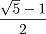
\includegraphics[keepaspectratio]{images/EMT4aljabar - Naila Khalidatus Salwa-045.png}}

Untuk menyelesaikan sistem persamaan, gunakan vektor persamaan. Hasilnya adalah vektor solusi.

\textgreater sol \&= solve({[}x+y=3,x\textsuperscript{2+y}2=5{]},{[}x,y{]}); \$\&sol, \$\&x*y with sol{[}1{]}

\[2\]\pandocbounded{
\includegraphics[keepaspectratio]{images/EMT4aljabar - Naila Khalidatus Salwa-047.png}}

Ekspresi simbolis dapat memiliki flag, yang menunjukkan perlakuan khusus di Maxima. Beberapa flag dapat digunakan sebagai perintah juga, yang lainnya tidak. Flag ditambahkan dengan ``\textbar{}'' (bentuk yang lebih bagus dari ``ev(\ldots,flags)'')

\textgreater\$\& diff((x\^{}3-1)/(x+1),x) //turunan bentuk pecahan

\[\frac{3\,x^2}{x+1}-\frac{x^3-1}{\left(x+1\right)^2}\]\textgreater\$\& diff((x\^{}3-1)/(x+1),x) \textbar{} ratsimp //menyederhanakan pecahan

\[\frac{2\,x^3+3\,x^2+1}{x^2+2\,x+1}\]\textgreater\$\&factor(\%)

\[\frac{2\,x^3+3\,x^2+1}{\left(x+1\right)^2}\]\# Contoh lainnya

\textgreater\$\& diff((3*x\^{}2-12*x+16),x)

\[6\,x-12\]\textgreater\$\&factor(\%)

\[6\,\left(x-2\right)\]\textgreater\$\&solve(-x\^{}2+6*x=8,x), x2 \&= x with \%{[}2{]}; \$\&x2

\[2\]\pandocbounded{
\includegraphics[keepaspectratio]{images/EMT4aljabar - Naila Khalidatus Salwa-054.png}}

\textgreater\&factor(8!)

\begin{verbatim}
                                40320
\end{verbatim}

\textgreater\$binomial(8,3) // C(8,3)

\[56\]\# Fungsi

Dalam EMT, fungsi adalah program yang didefinisikan dengan perintah ``function''. Ini bisa berupa fungsi satu baris atau fungsi multibaris.

Fungsi satu baris dapat berupa numerik atau simbolik. Fungsi satu baris numerik didefinisikan oleh ``:=''.

\textgreater function f(x) := x*sqrt(x\^{}2+1)

Untuk gambaran umum, kami menampilkan semua kemungkinan definisi untuk fungsi satu baris. Suatu fungsi dapat dievaluasi sama seperti fungsi Euler bawaan lainnya.

\textgreater f(2)

\begin{verbatim}
4.472135955
\end{verbatim}

Fungsi ini juga dapat digunakan untuk vektor, mengikuti bahasa matriks Euler, karena ekspresi yang digunakan dalam fungsi tersebut divektorkan.

\textgreater f(0:0.1:1)

\begin{verbatim}
[0,  0.100499,  0.203961,  0.313209,  0.430813,  0.559017,  0.699714,
0.854459,  1.0245,  1.21083,  1.41421]
\end{verbatim}

Fungsi dapat diplot. Daripada ekspresi, kita hanya perlu memberikan nama fungsinya.

Berbeda dengan ekspresi simbolik atau numerik, nama fungsi harus diberikan dalam string.

\textgreater solve(``f'',1,y=1)

\begin{verbatim}
0.786151377757
\end{verbatim}

Secara default, jika Anda perlu menimpa fungsi bawaan, Anda harus menambahkan kata kunci ``overwrite''. Menimpa fungsi bawaan berbahaya dan dapat menyebabkan masalah pada fungsi lain yang bergantung pada fungsi tersebut.

Anda masih dapat memanggil fungsi bawaan sebagai ``\_\ldots``, jika fungsi tersebut ada di inti Euler.

\textgreater function overwrite sin (x) := \_sin(x°) // redine sine in degrees

\textgreater sin(45)

\begin{verbatim}
0.707106781187
\end{verbatim}

Sebaiknya kita menghilangkan redefinisi sin ini.

\textgreater forget sin; sin(pi/4)

\chapter{Contoh lainnya}\label{contoh-lainnya-7}

\textgreater function f(x) := x\^{}2-6

\textgreater f(3)

\begin{verbatim}
  3.00000 
\end{verbatim}

\textgreater f(0:0.1:1)

\begin{verbatim}
Real 1 x 11 matrix

 -6.00000  -5.99000  -5.96000  -5.91000  -5.84000  -5.75000     ...
\end{verbatim}

\textgreater solve(``f'',1,y=3)

\begin{verbatim}
  3.00000 
\end{verbatim}

\textgreater function overwrite sin (x) := \_sin(x°) // redine sine in degrees

\textgreater sin(60)

\begin{verbatim}
  0.86603 
\end{verbatim}

\textgreater forget sin; sin(pi/3)

\begin{verbatim}
  0.86603 
\end{verbatim}

\section{Parameter Bawaan}\label{parameter-bawaan}

Fungsi numerik dapat memiliki parameter bawaan.

\textgreater function f(x,a=1) := a*x\^{}2

Menghilangkan parameter ini akan menggunakan nilai bawaan.

\textgreater f(4)

\begin{verbatim}
16
\end{verbatim}

Menyetelnya akan menimpa nilai default.

\textgreater f(4,5)

\begin{verbatim}
80
\end{verbatim}

Parameter yang ditetapkan akan menimpanya juga. Ini digunakan oleh banyak fungsi Euler seperti plot2d, plot3d.

\textgreater f(4,a=1)

\begin{verbatim}
16
\end{verbatim}

Jika suatu variabel bukan parameter, maka harus bersifat global. Fungsi satu baris dapat melihat variabel global.

\textgreater function f(x) := a*x\^{}2

\textgreater a=6; f(2)

\begin{verbatim}
24
\end{verbatim}

Namun parameter yang ditetapkan mengesampingkan nilai global.

Jika argumen tidak ada dalam daftar parameter yang telah ditentukan sebelumnya, argumen tersebut harus dideklarasikan dengan ``:=''!

\textgreater f(2,a:=5)

\begin{verbatim}
20
\end{verbatim}

Fungsi simbolik didefinisikan dengan ``\&=''. Mereka didefinisikan di Euler dan Maxima, dan bekerja di kedua dunia. Ekspresi yang didefinisikan dijalankan melalui Maxima sebelum definisi.

\textgreater function g(x) \&= x\^{}3-x*exp(-x); \$\&g(x)

Fungsi simbolik dapat digunakan dalam ekspresi simbolik.

\textgreater\$\&diff(g(x),x), \$\&\% with x=4/3

Mereka juga dapat digunakan dalam ekspresi numerik. Tentu saja, ini hanya akan berfungsi jika EMT dapat menafsirkan semua yang ada di dalam fungsi tersebut.

\textgreater g(5+g(1))

\begin{verbatim}
178.635099908
\end{verbatim}

Mereka dapat digunakan untuk mendefinisikan fungsi atau ekspresi simbolik lainnya.

\textgreater function G(x) \&= factor(integrate(g(x),x)); \$\&G(c) // integrate: mengintegralkan

\[\int {g\left(c\right)}{\;dc}\]\textgreater solve(\&g(x),0.5)

\begin{verbatim}
0.703467422498
\end{verbatim}

Berikut ini juga berfungsi, karena Euler menggunakan ekspresi simbolik dalam fungsi g, jika tidak menemukan variabel simbolik g, dan jika terdapat fungsi simbolik g.

\textgreater solve(\&g,0.5)

\begin{verbatim}
0.703467422498
\end{verbatim}

\textgreater function P(x,n) \&= (2*x-1)\^{}n; \$\&P(x,n)

\[\left(2\,x-1\right)^{n}\]\textgreater function Q(x,n) \&= (x+2)\^{}n; \$\&Q(x,n)

\[\left(x+2\right)^{n}\]\textgreater\$\&P(x,4), \$\&expand(\%)

\[16\,x^4-32\,x^3+24\,x^2-8\,x+1\]\pandocbounded{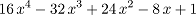
\includegraphics[keepaspectratio]{images/EMT4aljabar - Naila Khalidatus Salwa-060.png}}

\textgreater P(3,4)

\begin{verbatim}
625
\end{verbatim}

\textgreater\$\&P(x,4)+ Q(x,3), \$\&expand(\%)

\[P\left(x , 4\right)+Q\left(x , 3\right)\]\pandocbounded{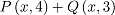
\includegraphics[keepaspectratio]{images/EMT4aljabar - Naila Khalidatus Salwa-062.png}}

\textgreater\$\&P(x,4)-Q(x,3), \$\&expand(\%), \$\&factor(\%)

\[16\,x^4-33\,x^3+18\,x^2-20\,x-7\]\pandocbounded{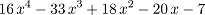
\includegraphics[keepaspectratio]{images/EMT4aljabar - Naila Khalidatus Salwa-064.png}}

\begin{figure}
\centering
\pandocbounded{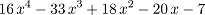
\includegraphics[keepaspectratio]{images/EMT4aljabar - Naila Khalidatus Salwa-065.png}}
\caption{images/EMT4aljabar\%20-\%20Naila\%20Khalidatus\%20Salwa-065.png}
\end{figure}

\textgreater\$\&P(x,4)*Q(x,3), \$\&expand(\%), \$\&factor(\%)

\[\left(x+2\right)^3\,\left(2\,x-1\right)^4\]\pandocbounded{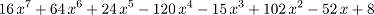
\includegraphics[keepaspectratio]{images/EMT4aljabar - Naila Khalidatus Salwa-067.png}}

\begin{figure}
\centering
\pandocbounded{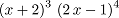
\includegraphics[keepaspectratio]{images/EMT4aljabar - Naila Khalidatus Salwa-068.png}}
\caption{images/EMT4aljabar\%20-\%20Naila\%20Khalidatus\%20Salwa-068.png}
\end{figure}

\textgreater\$\&P(x,4)/Q(x,1), \$\&expand(\%), \$\&factor(\%)

\[\frac{\left(2\,x-1\right)^4}{x+2}\]\pandocbounded{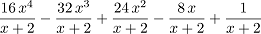
\includegraphics[keepaspectratio]{images/EMT4aljabar - Naila Khalidatus Salwa-070.png}}

\begin{figure}
\centering
\pandocbounded{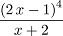
\includegraphics[keepaspectratio]{images/EMT4aljabar - Naila Khalidatus Salwa-071.png}}
\caption{images/EMT4aljabar\%20-\%20Naila\%20Khalidatus\%20Salwa-071.png}
\end{figure}

\textgreater function f(x) \&= x\^{}3-x; \$\&f(x)

\[x^3-x\]Dengan \&= fungsinya bersifat simbolis, dan dapat digunakan dalam ekspresi simbolik lainnya.

\textgreater\$\&integrate(f(x),x)

Dengan := fungsinya adalah numerik. Contoh yang baik adalah integral tentu

\[f(x) = \int_1^x t^t \, dt,\]yang tidak dapat dievaluasi secara simbolis.

Jika kita mendefinisikan ulang fungsi tersebut dengan kata kunci ``map'' maka dapat digunakan untuk vektor x. Secara internal, fungsi ini dipanggil untuk semua nilai x satu kali, dan hasilnya disimpan dalam vektor.

\textgreater function map f(x) := integrate(``x\^{}x'',1,x)

\textgreater f(0:0.5:2)

\begin{verbatim}
[-0.783431,  -0.410816,  0,  0.676863,  2.05045]
\end{verbatim}

Fungsi dapat memiliki nilai default untuk parameter.

\textgreater function mylog (x,base=10) := ln(x)/ln(base);

Sekarang fungsinya bisa dipanggil dengan atau tanpa parameter ``base''.

\textgreater mylog(100), mylog(2\^{}6.7,2)

\begin{verbatim}
2
6.7
\end{verbatim}

Selain itu, dimungkinkan untuk menggunakan parameter yang ditetapkan.

\textgreater mylog(E\^{}2,base=E)

\begin{verbatim}
2
\end{verbatim}

Seringkali, kita ingin menggunakan fungsi untuk vektor di satu tempat, dan untuk elemen individual di tempat lain. Hal ini dimungkinkan dengan parameter vektor.

\textgreater function f({[}a,b{]}) \&= a\textsuperscript{2+b}2-a*b+b; \$\&f(a,b), \$\&f(x,y)

Fungsi simbolik seperti ini dapat digunakan untuk variabel simbolik.

Namun fungsinya juga dapat digunakan untuk vektor numerik.

\textgreater v={[}3,4{]}; f(v)

\begin{verbatim}
17
\end{verbatim}

Ada juga fungsi yang murni simbolik, yang tidak dapat digunakan secara numerik.

\textgreater function lapl(expr,x,y) \&\&= diff(expr,x,2)+diff(expr,y,2)//turunan parsial kedua

\begin{verbatim}
                 diff(expr, y, 2) + diff(expr, x, 2)
\end{verbatim}

\textgreater\$\&realpart((x+I*y)\^{}4), \$\&lapl(\%,x,y)

\[{\it lapl}\left(y^4-6\,x^2\,y^2+x^4 , x , y\right)\]\pandocbounded{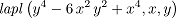
\includegraphics[keepaspectratio]{images/EMT4aljabar - Naila Khalidatus Salwa-075.png}}

Namun tentu saja, mereka dapat digunakan dalam ekspresi simbolik atau dalam definisi fungsi simbolik.

Untuk meringkas

\begin{itemize}
\item
  \&= mendefinisikan fungsi simbolik,
\item
  := mendefinisikan fungsi numerik,
\item
  \&\&= mendefinisikan fungsi simbolik murni.
\end{itemize}

\chapter{Contoh lainnya}\label{contoh-lainnya-8}

\textgreater function P(x,n) \&= x\^{}5-2=0; \$\&P(x,n)

\[x^5-2=0\]\textgreater function mylog (x,base=10) := ln(x)/ln(base);

\textgreater mylog(2\^{}2.8,3)

\begin{verbatim}
       1.77 
\end{verbatim}

\textgreater function F(x) \&= factor(integrate(f(x),x)); \$\&F(x)

\[\int {f\left(x\right)}{\;dx}\]\textgreater function f(x) \&= x\textsuperscript{3-5*x}2+3*x; \$\&f(x)

\[x^3-5\,x^2+3\,x\]\textgreater function f({[}a,b{]}) \&= a\textsuperscript{3+2*a}2-a*b+b; \$\&f(a,b)

\[-a\,b+b+a^3+2\,a^2\]\textgreater d={[}2,4{]}; f(d)

\begin{verbatim}
      12.00 
\end{verbatim}

\chapter{Memecahkan Ekspresi}\label{memecahkan-ekspresi}

Ekspresi dapat diselesaikan secara numerik dan simbolis.

Untuk menyelesaikan ekspresi sederhana dari satu variabel, kita dapat menggunakan fungsi solve(). Dibutuhkan nilai awal untuk memulai pencarian. Secara internal, solve() menggunakan metode secant.

\textgreater solve(``x\^{}2-2'',1)

\begin{verbatim}
1.41421356237
\end{verbatim}

Ini juga berfungsi untuk ekspresi simbolik. Ambil fungsi berikut.

\textgreater\$\&solve(x\^{}2=2,x)

\[\left[ x=-\sqrt{2} , x=\sqrt{2} \right] \]\textgreater\$\&solve(x\^{}2-2,x)

\[\left[ x=-\sqrt{2} , x=\sqrt{2} \right] \]\textgreater\$\&solve(a*x\^{}2+b*x+c=0,x)

\[\left[ x=\frac{-\sqrt{b^2-4\,a\,c}-b}{2\,a} , x=\frac{\sqrt{b^2-4\,  a\,c}-b}{2\,a} \right] \]\textgreater\$\&solve({[}a*x+b*y=c,d*x+e*y=f{]},{[}x,y{]})

\[\left[ \left[ x=\frac{b\,f-c\,e}{b\,d-a\,e} , y=\frac{c\,d-a\,f}{b  \,d-a\,e} \right]  \right] \]\textgreater px \&= 4*x\textsuperscript{8+x}7-x\^{}4-x; \$\&px

\[4\,x^8+x^7-x^4-x\]Sekarang kita mencari titik yang polinomialnya adalah 2. Dalam solve(), nilai target default y=0 dapat diubah dengan variabel yang ditetapkan.

Kami menggunakan y=2 dan memeriksa dengan mengevaluasi polinomial pada hasil sebelumnya.

\textgreater solve(px,1,y=2), px(\%)

\begin{verbatim}
0.966715594851
2
\end{verbatim}

Memecahkan ekspresi simbolik dalam bentuk simbolik mengembalikan daftar solusi. Kami menggunakan pemecah simbolis solve() yang disediakan oleh Maxima.

\textgreater sol \&= solve(x\^{}2-x-1,x); \$\&sol

Cara termudah untuk mendapatkan nilai numerik adalah dengan mengevaluasi solusi secara numerik seperti halnya ekspresi.

\textgreater longest sol()

\begin{verbatim}
    -0.6180339887498949       1.618033988749895 
\end{verbatim}

Untuk menggunakan solusi secara simbolis dalam ekspresi lain, cara termudah adalah dengan ``with''.

\textgreater{} \$\&x\^{}2 with sol {[}1{]}, \$\&expand(x\^{}2-x-1 with sol{[}2{]})

\[6-3\,\sqrt{5}\]\pandocbounded{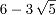
\includegraphics[keepaspectratio]{images/EMT4aljabar - Naila Khalidatus Salwa-086.png}}

Penyelesaian sistem persamaan secara simbolis dapat dilakukan dengan vektor persamaan dan solver simbolis solve(). Jawabannya adalah daftar daftar persamaan.

\textgreater\$\&solve({[}x+y=2,x\^{}3+2*y+x=4{]},{[}x,y{]})

\[\left[ \left[ x=-1 , y=3 \right]  , \left[ x=1 , y=1 \right]  ,   \left[ x=0 , y=2 \right]  \right] \]Fungsi f() dapat melihat variabel global. Namun seringkali kita ingin menggunakan parameter lokal.

\[a^x-x^a = 0.1\]dengan a=3.

\textgreater function f(x,a) := x\textsuperscript{a-a}x;

Salah satu cara untuk meneruskan parameter tambahan ke f() adalah dengan menggunakan daftar dengan nama fungsi dan parameternya (cara lainnya adalah parameter titik koma).

\textgreater solve(\{\{``f'',3\}\},2,y=0.1)

\begin{verbatim}
       2.54 
\end{verbatim}

Ini juga berfungsi dengan ekspresi. Namun kemudian, elemen daftar bernama harus digunakan. (Lebih lanjut tentang daftar di tutorial tentang sintaks EMT).

\textgreater solve(\{\{``x\textsuperscript{a-a}x'',a=3\}\},2,y=0.1)

\begin{verbatim}
  2.54116 
\end{verbatim}

\chapter{Contoh lainnya}\label{contoh-lainnya-9}

\textgreater\$\&solve(4\^{}x=8,x)

\[\left[ x=\frac{\log 8}{\log 4} \right] \]\textgreater\$\&solve (x\textsuperscript{2-x}4=5, x)

\[\left[ x=-\frac{\sqrt{\sqrt{19}\,i+1}}{\sqrt{2}} , x=\frac{\sqrt{  \sqrt{19}\,i+1}}{\sqrt{2}} , x=-\frac{\sqrt{1-\sqrt{19}\,i}}{\sqrt{2  }} , x=\frac{\sqrt{1-\sqrt{19}\,i}}{\sqrt{2}} \right] \]\textgreater\$\&solve(x\textsuperscript{3-2*x}2+x-24,x)

\[\left[ x=\frac{\frac{\sqrt{3}\,i}{2}-\frac{1}{2}}{9\,\left(\frac{2  \,\sqrt{322}}{3}+\frac{323}{27}\right)^{\frac{1}{3}}}+\left(\frac{2  \,\sqrt{322}}{3}+\frac{323}{27}\right)^{\frac{1}{3}}\,\left(-\frac{  \sqrt{3}\,i}{2}-\frac{1}{2}\right)+\frac{2}{3} , x=\left(\frac{2\,  \sqrt{322}}{3}+\frac{323}{27}\right)^{\frac{1}{3}}\,\left(\frac{  \sqrt{3}\,i}{2}-\frac{1}{2}\right)+\frac{-\frac{\sqrt{3}\,i}{2}-  \frac{1}{2}}{9\,\left(\frac{2\,\sqrt{322}}{3}+\frac{323}{27}\right)  ^{\frac{1}{3}}}+\frac{2}{3} , x=\left(\frac{2\,\sqrt{322}}{3}+\frac{  323}{27}\right)^{\frac{1}{3}}+\frac{1}{9\,\left(\frac{2\,\sqrt{322}  }{3}+\frac{323}{27}\right)^{\frac{1}{3}}}+\frac{2}{3} \right] \]\textgreater px \&= x\^{}2+5*x; \$\&px

\[x^2+5\,x\]\textgreater solve(px,1,y=2), px(\%)

\begin{verbatim}
  0.37228 
  2.00000 
\end{verbatim}

\section{Menyelesaikan Pertidaksamaan}\label{menyelesaikan-pertidaksamaan}

Untuk menyelesaikan pertidaksamaan, EMT tidak akan dapat melakukannya, melainkan dengan bantuan Maxima, artinya secara eksak (simbolik). Perintah Maxima yang digunakan adalah fourier\_elim(), yang harus dipanggil dengan perintah ``load(fourier\_elim)'' terlebih dahulu.

Eliminasi Fourier adalah analog dari eliminasi Gauss untuk linear (persamaan atau pertidaksamaan). Panggilan fungsi `fourier\_elim ({[}eq1,eq2,\ldots{]},{[}var1,var2,\ldots{]})' melakukan eliminasi Fourier dengan

\textgreater\&load(fourier\_elim)

\begin{verbatim}
       C:/Program Files/Euler x64/maxima/share/maxima/5.35.1/share/fo\
urier_elim/fourier_elim.lisp
\end{verbatim}

\textgreater\$\&fourier\_elim({[}x\^{}2 - 1\textgreater0{]},{[}x{]}) // x\^{}2-1 \textgreater{} 0

\[\left[ 1<x \right] \lor \left[ x<-1 \right] \]\textgreater\$\&fourier\_elim({[}x\^{}2 - 1\textless0{]},{[}x{]}) // x\^{}2-1 \textless{} 0

\[\left[ -1<x , x<1 \right] \]\textgreater\$\&fourier\_elim({[}x\^{}2 - 1 \# 0{]},{[}x{]}) // x\^{}-1 \textless\textgreater{} 0

\[\left[ -1<x , x<1 \right] \lor \left[ 1<x \right] \lor \left[ x<-1   \right] \]\textgreater\$\&fourier\_elim({[}x \# 6{]},{[}x{]})

\[\left[ x<6 \right] \lor \left[ 6<x \right] \]\textgreater\$\&fourier\_elim({[}x \textless{} 1, x \textgreater{} 1{]},{[}x{]}) // tidak memiliki penyelesaian

\[{\it emptyset}\]\textgreater\$\&fourier\_elim({[}minf \textless{} x, x \textless{} inf{]},{[}x{]}) // solusinya R

\[{\it universalset}\]\textgreater\$\&fourier\_elim({[}x\^{}3 - 1 \textgreater{} 0{]},{[}x{]})

\[\left[ 1<x , x^2+x+1>0 \right] \lor \left[ x<1 , -x^2-x-1>0   \right] \]\textgreater\$\&fourier\_elim({[}cos(x) \textless{} 1/2{]},{[}x{]}) // ??? gagal

\[\left[ 1-2\,\cos x>0 \right] \]\textgreater\$\&fourier\_elim({[}y-x \textless{} 5, x - y \textless{} 7, 10 \textless{} y{]},{[}x,y{]}) // sistem pertidaksamaan

\[\left[ y-5<x , x<y+7 , 10<y \right] \]\textgreater\$\&fourier\_elim({[}y-x \textless{} 5, x - y \textless{} 7, 10 \textless{} y{]},{[}y,x{]})

\[\left[ {\it max}\left(10 , x-7\right)<y , y<x+5 , 5<x \right] \]\textgreater\$\&fourier\_elim((x + y \textless{} 5) and (x - y \textgreater8),{[}x,y{]})

\[\left[ y+8<x , x<5-y , y<-\frac{3}{2} \right] \]\textgreater\$\&fourier\_elim(((x + y \textless{} 5) and x \textless{} 1) or (x - y \textgreater8),{[}x,y{]})

\[\left[ y+8<x \right] \lor \left[ x<{\it min}\left(1 , 5-y\right)   \right] \]\textgreater\&fourier\_elim({[}max(x,y) \textgreater{} 6, x \# 8, abs(y-1) \textgreater{} 12{]},{[}x,y{]})

\begin{verbatim}
        [6 &lt; x, x &lt; 8, y &lt; - 11] or [8 &lt; x, y &lt; - 11]
 or [x &lt; 8, 13 &lt; y] or [x = y, 13 &lt; y] or [8 &lt; x, x &lt; y, 13 &lt; y]
 or [y &lt; x, 13 &lt; y]
\end{verbatim}

\textgreater\$\&fourier\_elim({[}(x+6)/(x-9) \textless= 6{]},{[}x{]})

\[\left[ x=12 \right] \lor \left[ 12<x \right] \lor \left[ x<9   \right] \]\# Contoh Lainnya

Menyelesaikan pertidaksamaan

\[x+8 \le 9\]\textgreater\$\&fourier\_elim({[}x+8 \textless9{]},{[}x{]})

\[\left[ x<1 \right] \]\[x+6 \ge 7\]\textgreater\$\&fourier\_elim({[}x+6 \textgreater= 7{]},{[}x{]})

\[\left[ x=1 \right] \lor \left[ 1<x \right] \]\[2y - 3 \ge 1-y+5\]\textgreater\$\&fourier\_elim({[}2*y - 3\textgreater= 1-y+5{]},{[}y{]})

\[\left[ y=3 \right] \lor \left[ 3<y \right] \]\[(x-2)(x+5) > x(x-3)\]\textgreater\$\&fourier\_elim({[}(x-2)*(x+5) \textgreater x*(x-3){]},{[}x{]})

\[\left[ \frac{5}{3}<x \right] \]\[\frac {2x-1}{3} \ge \frac{5}{6}\]\textgreater\$\&fourier\_elim({[}(2*x-1)/3\textgreater= 5/6{]},{[}x{]})

\[\left[ x=\frac{7}{4} \right] \lor \left[ \frac{7}{4}<x \right] \]\# Bahasa Matriks

Dokumentasi inti EMT berisi pembahasan rinci tentang bahasa matriks Euler.

Vektor dan matriks dimasukkan dengan tanda kurung siku, elemen dipisahkan dengan koma, baris dipisahkan dengan titik koma.

\textgreater A={[}1,2;3,4{]}

\begin{verbatim}
            1             2 
            3             4 
\end{verbatim}

Hasil kali matriks dilambangkan dengan titik.

\textgreater b={[}3;4{]}

\begin{verbatim}
            3 
            4 
\end{verbatim}

Transpose matriks adalah matriks baru yang diperoleh dengan cara menukar elemen-elemen baris menjadi elemen kolom atau sebaliknya.

\textgreater b' // transpose b

\begin{verbatim}
[3,  4]
\end{verbatim}

Invers matriks adalah matriks baru yang merupakan kebalikan dari matriks asal

\textgreater inv(A) //inverse A

\begin{verbatim}
           -2             1 
          1.5          -0.5 
\end{verbatim}

Perkalian matriks sendiri adalah proses mengalikan setiap elemen baris pada matriks pertama dengan elemen kolom pada matriks kedua

\textgreater A.b //perkalian matriks

\begin{verbatim}
           11 
           25 
\end{verbatim}

Perkalian dari matriks dengan invers matriks sendiri itu akan menghasilkan matriks identitas

\textgreater A.inv(A)

\begin{verbatim}
            1             0 
            0             1 
\end{verbatim}

Poin utama dari bahasa matriks adalah semua fungsi dan operator bekerja elemen demi elemen.

Perkalian matriks dan perpangkatan matriks

\textgreater A.A

\begin{verbatim}
            7            10 
           15            22 
\end{verbatim}

\textgreater A\^{}2 //perpangkatan elemen2 A

\begin{verbatim}
            1             4 
            9            16 
\end{verbatim}

\textgreater A.A.A

\begin{verbatim}
           37            54 
           81           118 
\end{verbatim}

\textgreater power(A,3) //perpangkatan matriks

\begin{verbatim}
           37            54 
           81           118 
\end{verbatim}

Pembagian matriks

\textgreater A/A //pembagian elemen-elemen matriks yang seletak

\begin{verbatim}
            1             1 
            1             1 
\end{verbatim}

\textgreater A/b //pembagian elemen2 A oleh elemen2 b kolom demi kolom (karena b vektor kolom)

\begin{verbatim}
     0.333333      0.666667 
         0.75             1 
\end{verbatim}

Perkalian invers matriks dengan matriks lainnya

\textgreater A\textbackslash b // hasilkali invers A dan b, A\^{}(-1)b

\begin{verbatim}
           -2 
          2.5 
\end{verbatim}

\textgreater inv(A).b

\begin{verbatim}
           -2 
          2.5 
\end{verbatim}

\textgreater A\textbackslash A //A\^{}(-1)A

\begin{verbatim}
            1             0 
            0             1 
\end{verbatim}

\textgreater inv(A).A

\begin{verbatim}
            1             0 
            0             1 
\end{verbatim}

\textgreater A*A //perkalian elemen-elemen matriks seletak

\begin{verbatim}
            1             4 
            9            16 
\end{verbatim}

Ini bukan hasil kali matriks, melainkan perkalian elemen demi elemen. Hal yang sama juga berlaku untuk vektor.

\textgreater b\^{}2 // perpangkatan elemen-elemen matriks/vektor

\begin{verbatim}
            9 
           16 
\end{verbatim}

Jika salah satu operan adalah vektor atau skalar, maka operan tersebut diperluas secara alami.

\textgreater2*A

\begin{verbatim}
            2             4 
            6             8 
\end{verbatim}

Misalnya, jika operan adalah vektor kolom, elemennya diterapkan ke semua baris A.

\textgreater{[}1,2{]}*A

\begin{verbatim}
            1             4 
            3             8 
\end{verbatim}

Jika ini adalah vektor baris, maka diterapkan ke semua kolom A.

\textgreater A*{[}2,3{]}

\begin{verbatim}
            2             6 
            6            12 
\end{verbatim}

Kita dapat membayangkan perkalian ini seolah-olah vektor baris v telah diduplikasi untuk membentuk matriks yang berukuran sama dengan A.

\textgreater dup({[}1,2{]},2) // dup: menduplikasi/menggandakan vektor {[}1,2{]} sebanyak 2 kali (baris)

\begin{verbatim}
            1             2 
            1             2 
\end{verbatim}

\textgreater A*dup({[}1,2{]},2)

\begin{verbatim}
            1             4 
            3             8 
\end{verbatim}

Hal ini juga berlaku untuk dua vektor dimana yang satu adalah vektor baris dan yang lainnya adalah vektor kolom. Kita menghitung i*j untuk i,j dari 1 sampai 5. Caranya adalah dengan mengalikan 1:5 dengan transposenya. Bahasa matriks Euler secara otomatis menghasilkan tabel nilai.

\textgreater(1:5)*(1:5)' // hasilkali elemen-elemen vektor baris dan vektor kolom

\begin{verbatim}
            1             2             3             4             5 
            2             4             6             8            10 
            3             6             9            12            15 
            4             8            12            16            20 
            5            10            15            20            25 
\end{verbatim}

Sekali lagi, ingatlah bahwa ini bukan produk matriks!

\textgreater(1:5).(1:5)' // hasilkali vektor baris dan vektor kolom

\begin{verbatim}
55
\end{verbatim}

\textgreater sum((1:5)*(1:5)) // sama hasilnya

\begin{verbatim}
55
\end{verbatim}

Bahkan operator seperti \textless{} atau == bekerja dengan cara yang sama.

\textgreater(1:10)\textless6 // menguji elemen-elemen yang kurang dari 6

\begin{verbatim}
[1,  1,  1,  1,  1,  0,  0,  0,  0,  0]
\end{verbatim}

Misalnya, kita dapat menghitung jumlah elemen yang memenuhi kondisi tertentu dengan fungsi sum().

\textgreater sum((1:10)\textless6) // banyak elemen yang kurang dari 6

\begin{verbatim}
5
\end{verbatim}

Euler memiliki operator perbandingan, seperti ``=='', yang memeriksa persamaan.

Kita mendapatkan vektor 0 dan 1, dimana 1 berarti benar.

\textgreater t=(1:10)\^{}2; t==25 //menguji elemen2 t yang sama dengan 25 (hanya ada 1)

\begin{verbatim}
[0,  0,  0,  0,  1,  0,  0,  0,  0,  0]
\end{verbatim}

Dari vektor tersebut, ``nonzeros'' memilih elemen bukan nol.

Dalam hal ini, kita mendapatkan indeks semua elemen lebih besar dari 50.

\textgreater nonzeros(t\textgreater50) //indeks elemen2 t yang lebih besar daripada 50

\begin{verbatim}
[8,  9,  10]
\end{verbatim}

Tentu saja, kita dapat menggunakan vektor indeks ini untuk mendapatkan nilai yang sesuai dalam t.

\textgreater t{[}nonzeros(t\textgreater50){]} //elemen2 t yang lebih besar daripada 50

\begin{verbatim}
[64,  81,  100]
\end{verbatim}

Sebagai contoh, mari kita cari semua kuadrat bilangan 1 sampai 1000, yang memenuhi 5 modulo 11 dan 3 modulo 13.

\textgreater t=1:1000; nonzeros(mod(t\^{}2,11)==5 \&\& mod(t\^{}2,13)==3)

\begin{verbatim}
[4,  48,  95,  139,  147,  191,  238,  282,  290,  334,  381,  425,
433,  477,  524,  568,  576,  620,  667,  711,  719,  763,  810,  854,
862,  906,  953,  997]
\end{verbatim}

EMT tidak sepenuhnya efektif untuk perhitungan bilangan bulat. Ia menggunakan floating point presisi ganda secara internal. Namun, seringkali hal ini sangat berguna.

Kita dapat memeriksa primalitasnya. Mari kita cari tahu, berapa banyak persegi ditambah 1 yang merupakan bilangan prima.

\textgreater t=1:1000; length(nonzeros(isprime(t\^{}2+1)))

\begin{verbatim}
112
\end{verbatim}

Fungsi nonzeros() hanya berfungsi untuk vektor. Untuk matriks, menggunakan mnonzeros().

\textgreater seed(2); A=random(3,4)

\begin{verbatim}
     0.765761      0.401188      0.406347      0.267829 
      0.13673      0.390567      0.495975      0.952814 
     0.548138      0.006085      0.444255      0.539246 
\end{verbatim}

Ini mengembalikan indeks elemen, yang bukan nol.

\textgreater k=mnonzeros(A\textless0.4) //indeks elemen2 A yang kurang dari 0,4

\begin{verbatim}
            1             4 
            2             1 
            2             2 
            3             2 
\end{verbatim}

Indeks ini dapat digunakan untuk mengatur elemen ke nilai tertentu.

\textgreater mset(A,k,0) //mengganti elemen2 suatu matriks pada indeks tertentu

\begin{verbatim}
     0.765761      0.401188      0.406347             0 
            0             0      0.495975      0.952814 
     0.548138             0      0.444255      0.539246 
\end{verbatim}

Fungsi mset() juga dapat mengatur elemen pada indeks ke entri beberapa matriks lainnya.

\textgreater mset(A,k,-random(size(A)))

\begin{verbatim}
     0.765761      0.401188      0.406347     -0.126917 
    -0.122404     -0.691673      0.495975      0.952814 
     0.548138     -0.483902      0.444255      0.539246 
\end{verbatim}

Dan dimungkinkan untuk mendapatkan elemen dalam vektor.

\textgreater mget(A,k)

\begin{verbatim}
[0.267829,  0.13673,  0.390567,  0.006085]
\end{verbatim}

Fungsi lain yang berguna adalah ekstrem, yang mengembalikan nilai minimal dan maksimal di setiap baris matriks dan posisinya.

\textgreater ex=extrema(A)

\begin{verbatim}
     0.267829             4      0.765761             1 
      0.13673             1      0.952814             4 
     0.006085             2      0.548138             1 
\end{verbatim}

Kita dapat menggunakan ini untuk mengekstrak nilai maksimal di setiap baris.

\textgreater ex{[},3{]}'

\begin{verbatim}
[0.765761,  0.952814,  0.548138]
\end{verbatim}

Ini tentu saja sama dengan fungsi max().

\textgreater max(A)'

\begin{verbatim}
[0.765761,  0.952814,  0.548138]
\end{verbatim}

Namun dengan mget(), kita dapat mengekstrak indeks dan menggunakan informasi ini untuk mengekstrak elemen pada posisi yang sama dari matriks lain.

\textgreater j=(1:rows(A))'\textbar ex{[},4{]}, mget(-A,j)

\chapter{Contoh lainnya}\label{contoh-lainnya-10}

Tentukan nilai-nilai yang diminta pada soal di bawah ini

\textgreater A={[}1,2;4,3{]}

\begin{verbatim}
            1             2 
            4             3 
\end{verbatim}

\textgreater B ={[}-3,5;2,-1{]}

\begin{verbatim}
           -3             5 
            2            -1 
\end{verbatim}

\[A+B\]\textgreater A+B

\begin{verbatim}
           -2             7 
            6             2 
\end{verbatim}

\[A-B\]\textgreater A-B

\begin{verbatim}
            4            -3 
            2             4 
\end{verbatim}

\[B\times A\]\textgreater B*A

\begin{verbatim}
           -3            10 
            8            -3 
\end{verbatim}

\[2 \times A\]\textgreater2*A

\begin{verbatim}
            2             4 
            8             6 
\end{verbatim}

\[B+A\]\textgreater B+A

\begin{verbatim}
           -2             7 
            6             2 
\end{verbatim}

\chapter{Fungsi Matriks Lainnya (Building Matriks)}\label{fungsi-matriks-lainnya-building-matriks}

Untuk membangun sebuah matriks, kita dapat menumpuk satu matriks di atas matriks lainnya. Jika keduanya tidak memiliki jumlah kolom yang sama, maka kolom yang lebih pendek akan diisi dengan 0.

\textgreater v=1:3; v\_v

\begin{verbatim}
            1             2             3 
            1             2             3 
\end{verbatim}

Demikian pula, kita dapat melampirkan matriks ke matriks lain secara berdampingan, jika keduanya mempunyai jumlah baris yang sama.

\textgreater A=random(3,4); A\textbar v'

\begin{verbatim}
     0.655416      0.200995      0.893622      0.281887             1 
        0.525      0.314127      0.444616      0.299474             2 
      0.28269      0.883227      0.270906      0.704419             3 
\end{verbatim}

Jika jumlah barisnya tidak sama, matriks yang lebih pendek diisi dengan 0.

Ada pengecualian untuk aturan ini. Bilangan real yang melekat pada suatu matriks akan digunakan sebagai kolom yang diisi dengan bilangan real tersebut.

\textgreater A\textbar1

\begin{verbatim}
     0.655416      0.200995      0.893622      0.281887             1 
        0.525      0.314127      0.444616      0.299474             1 
      0.28269      0.883227      0.270906      0.704419             1 
\end{verbatim}

Dimungkinkan untuk membuat matriks vektor baris dan kolom.

\textgreater{[}v;v{]}

\begin{verbatim}
            1             2             3 
            1             2             3 
\end{verbatim}

\textgreater{[}v,v{]}

\begin{verbatim}
[1,  2,  3,  1,  2,  3]
\end{verbatim}

\textgreater{[}v',v'{]}

\begin{verbatim}
            1             1 
            2             2 
            3             3 
\end{verbatim}

Tujuan utamanya adalah untuk menafsirkan ekspresi vektor untuk vektor kolom.

\textgreater{}``{[}x,x\^{}2{]}''(v')

\begin{verbatim}
            1             1 
            2             4 
            3             9 
\end{verbatim}

Untuk mendapatkan ukuran A, kita bisa menggunakan fungsi berikut.

\textgreater C=zeros(2,4); rows(C), cols(C), size(C), length(C)

\begin{verbatim}
2
4
[2,  4]
4
\end{verbatim}

Untuk vektor, ada length().

\textgreater length(2:10)

\begin{verbatim}
9
\end{verbatim}

Masih banyak fungsi lain yang menghasilkan matriks.

\textgreater ones(2,2)

\begin{verbatim}
            1             1 
            1             1 
\end{verbatim}

Ini juga dapat digunakan dengan satu parameter. Untuk mendapatkan vektor dengan bilangan selain 1, gunakan yang berikut ini.

\textgreater ones(5)*6

\begin{verbatim}
[6,  6,  6,  6,  6]
\end{verbatim}

Matriks bilangan acak juga dapat dihasilkan dengan acak (distribusi seragam) atau normal (distribusi Gauß).

\textgreater random(2,2)

\begin{verbatim}
      0.66566      0.831835 
        0.977      0.544258 
\end{verbatim}

Berikut adalah fungsi lain yang berguna, yang merestrukturisasi elemen matriks menjadi matriks lain.

\textgreater redim(1:9,3,3) // menyusun elemen2 1, 2, 3, \ldots, 9 ke bentuk matriks 3x3

\begin{verbatim}
            1             2             3 
            4             5             6 
            7             8             9 
\end{verbatim}

Dengan fungsi berikut, kita dapat menggunakan fungsi ini dan fungsi dup untuk menulis fungsi rep(), yang mengulangi vektor sebanyak n kali.

\textgreater function rep(v,n) := redim(dup(v,n),1,n*cols(v))

Mari kita coba.

\textgreater rep(1:3,5)

\begin{verbatim}
[1,  2,  3,  1,  2,  3,  1,  2,  3,  1,  2,  3,  1,  2,  3]
\end{verbatim}

Fungsi multdup() menduplikasi elemen vektor.

\textgreater multdup(1:3,5), multdup(1:3,{[}2,3,2{]})

\begin{verbatim}
[1,  1,  1,  1,  1,  2,  2,  2,  2,  2,  3,  3,  3,  3,  3]
[1,  1,  2,  2,  2,  3,  3]
\end{verbatim}

Fungsi flipx() dan flipy() mengembalikan urutan baris atau kolom matriks. Yaitu, fungsi flipx() membalik secara horizontal.

Jika jumlah kolom tidak sama, kolom yang lebih pendek akan diisi 0.

\textgreater flipx(1:5) //membalik elemen2 vektor baris

\begin{verbatim}
[5,  4,  3,  2,  1]
\end{verbatim}

Untuk rotasi, Euler memiliki rotleft() dan rotright().

\textgreater rotleft(1:5) // memutar elemen2 vektor baris

\begin{verbatim}
[2,  3,  4,  5,  1]
\end{verbatim}

Fungsi khusus adalah drop(v,i), yang menghilangkan elemen dengan indeks di i dari vektor v.

\textgreater drop(10:20,3)

\begin{verbatim}
[10,  11,  13,  14,  15,  16,  17,  18,  19,  20]
\end{verbatim}

Perhatikan bahwa vektor i di drop(v,i) mengacu pada indeks elemen di v, bukan nilai elemen. Jika Anda ingin menghapus elemen, Anda perlu mencari elemennya terlebih dahulu. Fungsi indexof(v,x) dapat digunakan untuk mencari elemen x dalam vektor yang diurutkan v.

\textgreater v=primes(50), i=indexof(v,10:20), drop(v,i)

\begin{verbatim}
[2,  3,  5,  7,  11,  13,  17,  19,  23,  29,  31,  37,  41,  43,  47]
[0,  5,  0,  6,  0,  0,  0,  7,  0,  8,  0]
[2,  3,  5,  7,  23,  29,  31,  37,  41,  43,  47]
\end{verbatim}

Seperti yang Anda lihat, tidak ada salahnya memasukkan indeks di luar rentang (seperti 0), indeks ganda, atau indeks yang tidak diurutkan.

\textgreater drop(1:10,shuffle({[}0,0,5,5,7,12,12{]}))

\begin{verbatim}
[1,  2,  3,  4,  6,  8,  9,  10]
\end{verbatim}

Ada beberapa fungsi khusus untuk mengatur diagonal atau menghasilkan matriks diagonal.

Kita mulai dengan matriks identitas.

\textgreater A=id(5) // matriks identitas 5x5

\begin{verbatim}
            1             0             0             0             0 
            0             1             0             0             0 
            0             0             1             0             0 
            0             0             0             1             0 
            0             0             0             0             1 
\end{verbatim}

Kemudian kita atur diagonal bawah (-1) menjadi 1:4.

\textgreater setdiag(A,-1,1:4) //mengganti diagonal di bawah diagonal utama

\begin{verbatim}
            1             0             0             0             0 
            1             1             0             0             0 
            0             2             1             0             0 
            0             0             3             1             0 
            0             0             0             4             1 
\end{verbatim}

Perhatikan bahwa kami tidak mengubah matriks A. Kami mendapatkan matriks baru sebagai hasil dari setdiag().

Berikut adalah fungsi yang mengembalikan matriks tri-diagonal.

\textgreater function tridiag (n,a,b,c) := setdiag(setdiag(b*id(n),1,c),-1,a); \ldots{}\\
\textgreater{} tridiag(5,1,2,3)

\begin{verbatim}
            2             3             0             0             0 
            1             2             3             0             0 
            0             1             2             3             0 
            0             0             1             2             3 
            0             0             0             1             2 
\end{verbatim}

Diagonal suatu matriks juga dapat diekstraksi dari matriks tersebut. Untuk mendemonstrasikannya, kami menyusun ulang vektor 1:9 menjadi matriks 3x3.

\textgreater A=redim(1:9,3,3)

\begin{verbatim}
            1             2             3 
            4             5             6 
            7             8             9 
\end{verbatim}

Sekarang kita dapat mengekstrak diagonalnya.

\textgreater d=getdiag(A,0)

\begin{verbatim}
[1,  5,  9]
\end{verbatim}

Misalnya. Kita dapat membagi matriks dengan diagonalnya. Bahasa matriks menjaga agar vektor kolom d diterapkan pada matriks baris demi baris.

\textgreater fraction A/d'

\begin{verbatim}
        1         2         3 
      4/5         1       6/5 
      7/9       8/9         1 
\end{verbatim}

\chapter{Contoh lainnya}\label{contoh-lainnya-11}

\textgreater I=id(2)

\begin{verbatim}
            1             0 
            0             1 
\end{verbatim}

\textgreater A=redim(1:8,4,2)

\begin{verbatim}
            1             2 
            3             4 
            5             6 
            7             8 
\end{verbatim}

\textgreater random(3,3)

\begin{verbatim}
     0.655416      0.200995      0.893622 
     0.281887         0.525      0.314127 
     0.444616      0.299474       0.28269 
\end{verbatim}

\textgreater drop(1:20,4)

\begin{verbatim}
[1,  2,  3,  5,  6,  7,  8,  9,  10,  11,  12,  13,  14,  15,  16,  17,
18,  19,  20]
\end{verbatim}

\textgreater{} rotleft(5:15)

\begin{verbatim}
[6,  7,  8,  9,  10,  11,  12,  13,  14,  15,  5]
\end{verbatim}

\chapter{Vektorisasi}\label{vektorisasi}

Hampir semua fungsi di Euler juga berfungsi untuk input matriks dan vektor, jika hal ini masuk akal.

Misalnya, fungsi sqrt() menghitung akar kuadrat dari semua elemen vektor atau matriks.

\textgreater sqrt(1:3)

\begin{verbatim}
[1,  1.41421,  1.73205]
\end{verbatim}

Jadi Anda dapat dengan mudah membuat tabel nilai. Ini adalah salah satu cara untuk memplot suatu fungsi (alternatifnya menggunakan ekspresi).

\textgreater x=1:0.01:5; y=log(x)/x\^{}2; // terlalu panjang untuk ditampikan

Dengan ini dan operator titik dua a:delta:b, vektor nilai fungsi dapat dihasilkan dengan mudah.

Pada contoh berikut, kita menghasilkan vektor nilai t{[}i{]} dengan jarak 0,1 dari -1 hingga 1. Kemudian kita menghasilkan vektor nilai fungsi

\[s = t^3-t\]\textgreater t=-1:0.1:1; s=t\^{}3-t

\begin{verbatim}
[0,  0.171,  0.288,  0.357,  0.384,  0.375,  0.336,  0.273,  0.192,
0.099,  0,  -0.099,  -0.192,  -0.273,  -0.336,  -0.375,  -0.384,
-0.357,  -0.288,  -0.171,  0]
\end{verbatim}

EMT memperluas operator untuk skalar, vektor, dan matriks dengan cara yang jelas.

Misalnya, vektor kolom dikali vektor baris diekspansi ke matriks, jika operator diterapkan. Berikut ini, v' adalah vektor yang dialihkan (vektor kolom).

\textgreater shortest (1:5)*(1:5)'

\begin{verbatim}
     1      2      3      4      5 
     2      4      6      8     10 
     3      6      9     12     15 
     4      8     12     16     20 
     5     10     15     20     25 
\end{verbatim}

Perhatikan, ini sangat berbeda dengan perkalian matriks. Hasil kali matriks dilambangkan dengan titik ``.'' di EMT.

\textgreater(1:5).(1:5)'

\begin{verbatim}
55
\end{verbatim}

Secara default, vektor baris dicetak dalam format ringkas.

\textgreater{[}1,2,3,4{]}

\begin{verbatim}
[1,  2,  3,  4]
\end{verbatim}

Untuk matriks operator khusus . menunjukkan perkalian matriks, dan A' menunjukkan transposisi. Matriks 1x1 dapat digunakan seperti bilangan real.

\textgreater v:={[}1,2{]}; v.v', \%\^{}2

\begin{verbatim}
5
25
\end{verbatim}

Untuk mengubah urutan matriks kita menggunakan apostrof.

\textgreater v=1:4; v'

\begin{verbatim}
            1 
            2 
            3 
            4 
\end{verbatim}

Jadi kita dapat menghitung matriks A dikalikan vektor b.

\textgreater A={[}1,2,3,4;5,6,7,8{]}; A.v'

\begin{verbatim}
           30 
           70 
\end{verbatim}

Perhatikan bahwa v masih merupakan vektor baris. Jadi v'.v berbeda dengan v.v'.

\textgreater v'.v

\begin{verbatim}
            1             2             3             4 
            2             4             6             8 
            3             6             9            12 
            4             8            12            16 
\end{verbatim}

v.v' menghitung norma v kuadrat untuk vektor baris v. Hasilnya adalah vektor 1x1, yang berfungsi seperti bilangan real.

\textgreater v.v'

\begin{verbatim}
30
\end{verbatim}

Ada juga fungsi norma (bersama dengan banyak fungsi Aljabar Linier lainnya).

\textgreater norm(v)\^{}2

\begin{verbatim}
30
\end{verbatim}

Operator dan fungsi mematuhi bahasa matriks Euler.

Berikut ringkasan peraturannya.

\begin{itemize}
\item
  Suatu fungsi yang diterapkan pada vektor atau matriks diterapkan
\item
  pada setiap elemen.
\item
  Operator yang mengoperasikan dua matriks dengan ukuran yang sama
\item
  diterapkan secara berpasangan pada elemen-elemen matriks.
\item
  Jika kedua matriks mempunyai dimensi yang berbeda, keduanya
\item
  diekspansi secara rasional sehingga mempunyai ukuran yang sama.
\end{itemize}

Misalnya, nilai skalar dikalikan vektor dengan mengalikan nilai setiap elemen vektor. Atau matriks dikalikan vektor (dengan *, bukan .) memperluas vektor ke ukuran matriks dengan menduplikasinya.

Berikut ini adalah kasus sederhana dengan operator \^{}.

\textgreater{[}1,2,3{]}\^{}2

\begin{verbatim}
[1,  4,  9]
\end{verbatim}

Ini kasus yang lebih rumit. Vektor baris dikalikan vektor kolom memperluas keduanya dengan cara menduplikasi.

\textgreater v:={[}1,2,3{]}; v*v'

\begin{verbatim}
            1             2             3 
            2             4             6 
            3             6             9 
\end{verbatim}

Perhatikan bahwa perkalian skalar menggunakan perkalian matriks, bukan *!

\textgreater v.v'

\begin{verbatim}
14
\end{verbatim}

Ada banyak fungsi matriks. Kami memberikan daftar singkat. Anda harus membaca dokumentasi untuk informasi lebih lanjut tentang perintah ini.

sum,prod menghitung jumlah dan hasil kali baris\\
cumsum,cumprod melakukan hal yang sama secara kumulatif\\
menghitung nilai ekstrem setiap baris\\
extreme mengembalikan vektor dengan informasi ekstrem\\
diag(A,i) mengembalikan diagonal ke-i\\
setdiag(A,i,v) mengatur diagonal ke-i\\
id(n) matriks identitas\\
det(A) determinan\\
charpoly(A) polinomial karakteristik\\
eigenvalues(A) nilai eigen

\textgreater v*v, sum(v*v), cumsum(v*v)

\begin{verbatim}
[1,  4,  9]
14
[1,  5,  14]
\end{verbatim}

Operator : menghasilkan vektor baris dengan spasi yang sama, opsional dengan ukuran langkah.

\textgreater1:4, 1:2:10

\begin{verbatim}
[1,  2,  3,  4]
[1,  3,  5,  7,  9]
\end{verbatim}

Untuk menggabungkan matriks dan vektor terdapat operator ``\textbar{}'' dan ``\_``.

\textgreater{[}1,2,3{]}\textbar{[}4,5{]}, {[}1,2,3{]}\_1

\begin{verbatim}
[1,  2,  3,  4,  5]
            1             2             3 
            1             1             1 
\end{verbatim}

Elemen-elemen matriks disebut dengan ``A{[}i,j{]}''.

\textgreater A:={[}1,2,3;4,5,6;7,8,9{]}; A{[}2,3{]}

\begin{verbatim}
6
\end{verbatim}

Untuk vektor baris atau kolom, v{[}i{]} adalah elemen ke-i dari vektor tersebut. Untuk matriks, ini mengembalikan baris ke-i yang lengkap dari matriks tersebut.

\textgreater v:={[}2,4,6,8{]}; v{[}3{]}, A{[}3{]}

\begin{verbatim}
6
[7,  8,  9]
\end{verbatim}

Indeks juga dapat berupa vektor baris dari indeks. : menunjukkan semua indeks.

\textgreater v{[}1:2{]}, A{[}:,2{]}

\begin{verbatim}
[2,  4]
            2 
            5 
            8 
\end{verbatim}

Bentuk kependekan dari : menghilangkan indeks sepenuhnya.

\textgreater A{[},2:3{]}

\begin{verbatim}
            2             3 
            5             6 
            8             9 
\end{verbatim}

Untuk tujuan vektorisasi, elemen matriks dapat diakses seolah-olah elemen tersebut adalah vektor.

\textgreater A\{4\}

\begin{verbatim}
4
\end{verbatim}

Matriks juga dapat diratakan menggunakan fungsi redim(). Ini diimplementasikan dalam fungsi flatten().

\textgreater redim(A,1,prod(size(A))), flatten(A)

\begin{verbatim}
[1,  2,  3,  4,  5,  6,  7,  8,  9]
[1,  2,  3,  4,  5,  6,  7,  8,  9]
\end{verbatim}

Untuk menggunakan matriks pada tabel, mari kita atur ulang ke format default, dan hitung tabel nilai sinus dan kosinus. Perhatikan bahwa sudut dinyatakan dalam radian secara default.

\textgreater defformat; w=0°:45°:360°; w=w'; deg(w)

\begin{verbatim}
            0 
           45 
           90 
          135 
          180 
          225 
          270 
          315 
          360 
\end{verbatim}

Sekarang kita menambahkan kolom ke matriks.

\textgreater M = deg(w)\textbar w\textbar cos(w)\textbar sin(w)

\begin{verbatim}
            0             0             1             0 
           45      0.785398      0.707107      0.707107 
           90        1.5708             0             1 
          135       2.35619     -0.707107      0.707107 
          180       3.14159            -1             0 
          225       3.92699     -0.707107     -0.707107 
          270       4.71239             0            -1 
          315       5.49779      0.707107     -0.707107 
          360       6.28319             1             0 
\end{verbatim}

Dengan menggunakan bahasa matriks, kita dapat menghasilkan beberapa tabel dari beberapa fungsi sekaligus.

Dalam contoh berikut, kita menghitung t{[}j{]}\^{}i untuk i dari 1 hingga n. Kita mendapatkan sebuah matriks, yang setiap barisnya merupakan tabel t\^{}i untuk satu i. Artinya, matriks memiliki elemen latex: a\_\{i,j\} = t\_j\^{}i, \quad 1 \le j \le 101, \quad 1 \le i \le n

Fungsi yang tidak berfungsi untuk masukan vektor harus ``divektorkan''. Hal ini dapat dicapai dengan kata kunci ``map'' dalam definisi fungsi. Kemudian fungsi tersebut akan dievaluasi untuk setiap elemen parameter vektor.

Integrasi numerik integral() hanya berfungsi untuk batas interval skalar. Jadi kita perlu membuat vektorisasinya.

\textgreater function map f(x) := integrate(``x\^{}x'',1,x)

Kata kunci ``map'' membuat vektorisasi fungsi tersebut. Fungsinya sekarang akan berfungsi untuk vektor bilangan.

\textgreater f({[}1:5{]})

\begin{verbatim}
[0,  2.05045,  13.7251,  113.336,  1241.03]
\end{verbatim}

\chapter{Contoh lainnya}\label{contoh-lainnya-12}

\textgreater F={[}3,3 ;-1,-1{]}

\begin{verbatim}
            3             3 
           -1            -1 
\end{verbatim}

\textgreater F'

\begin{verbatim}
            3            -1 
            3            -1 
\end{verbatim}

\textgreater F*F'

\begin{verbatim}
            9            -3 
           -3             1 
\end{verbatim}

\textgreater sum(F*F')

\begin{verbatim}
            6 
           -2 
\end{verbatim}

\textgreater defformat; g=0°:30°:180°; g=g'; deg(g)

\begin{verbatim}
            0 
           30 
           60 
           90 
          120 
          150 
          180 
\end{verbatim}

\chapter{Sub-Matriks dan Matriks-Elemen}\label{sub-matriks-dan-matriks-elemen}

Untuk mengakses elemen matriks, gunakan notasi braket.

\textgreater A={[}1,2,3;4,5,6;7,8,9{]}, A{[}2,2{]}

\begin{verbatim}
            1             2             3 
            4             5             6 
            7             8             9 
5
\end{verbatim}

Kita dapat mengakses baris matriks secara lengkap.

\textgreater A{[}2{]}

\begin{verbatim}
[4,  5,  6]
\end{verbatim}

Dalam kasus vektor baris atau kolom, ini mengembalikan elemen vektor.

\textgreater v=1:3; v{[}2{]}

\begin{verbatim}
2
\end{verbatim}

Untuk memastikan, Anda mendapatkan baris pertama untuk matriks 1xn dan mxn, tentukan semua kolom menggunakan indeks kedua yang kosong.

\textgreater A{[}2,{]}

\begin{verbatim}
[4,  5,  6]
\end{verbatim}

Jika indeks adalah vektor dari indeks, Euler akan mengembalikan baris matriks yang sesuai.

Di sini kita menginginkan baris pertama dan kedua A.

\begin{verbatim}
            1             2             3 
            4             5             6 
\end{verbatim}

Kita bahkan dapat menyusun ulang A menggunakan vektor indeks. Tepatnya, kita tidak mengubah A di sini, namun menghitung versi A yang disusun ulang.

\begin{verbatim}
            7             8             9 
            4             5             6 
            1             2             3 
\end{verbatim}

Trik indeks berfungsi juga untuk kolom.

Contoh ini memilih semua baris A dan kolom kedua dan ketiga.

\textgreater A{[}1:3,2:3{]}

\begin{verbatim}
            2             3 
            5             6 
            8             9 
\end{verbatim}

Untuk singkatan ``:'' menunjukkan semua indeks baris atau kolom.

\textgreater A{[}:,3{]}

\begin{verbatim}
            3 
            6 
            9 
\end{verbatim}

Alternatifnya, biarkan indeks pertama kosong.

\textgreater A{[},2:3{]}

\begin{verbatim}
            2             3 
            5             6 
            8             9 
\end{verbatim}

Kita juga bisa mendapatkan baris terakhir A.

\textgreater A{[}-1{]}

\begin{verbatim}
[7,  8,  9]
\end{verbatim}

Sekarang mari kita ubah elemen A dengan menetapkan submatriks A ke beberapa nilai. Ini sebenarnya mengubah matriks A yang disimpan.

\textgreater A{[}1,1{]}=4

\begin{verbatim}
            4             2             3 
            4             5             6 
            7             8             9 
\end{verbatim}

Kita juga dapat memberikan nilai pada baris A.

\textgreater A{[}1{]}={[}-1,-1,-1{]}

\begin{verbatim}
           -1            -1            -1 
            4             5             6 
            7             8             9 
\end{verbatim}

Kita bahkan dapat menetapkan sub-matriks jika ukurannya sesuai.

\textgreater A{[}1:2,1:2{]}={[}5,6;7,8{]}

\begin{verbatim}
            5             6            -1 
            7             8             6 
            7             8             9 
\end{verbatim}

Selain itu, beberapa jalan pintas diperbolehkan.

\textgreater A{[}1:2,1:2{]}=0

\begin{verbatim}
            0             0            -1 
            0             0             6 
            7             8             9 
\end{verbatim}

Peringatan: Indeks di luar batas mengembalikan matriks kosong, atau pesan kesalahan, bergantung pada pengaturan sistem. Standarnya adalah pesan kesalahan. Namun perlu diingat bahwa indeks negatif dapat digunakan untuk mengakses elemen matriks yang dihitung dari akhir.

\textgreater A{[}4{]}

\begin{verbatim}
Row index 4 out of bounds!
Error in:
A[4] ...
    ^
\end{verbatim}

\chapter{Contoh Lainnya}\label{contoh-lainnya-13}

\textgreater A={[}-3,1,0; 0,2,-1; 5,0,4{]}

\begin{verbatim}
           -3             1             0 
            0             2            -1 
            5             0             4 
\end{verbatim}

\textgreater A{[}2{]}

\begin{verbatim}
[0,  2,  -1]
\end{verbatim}

\begin{verbatim}
            0             2            -1 
            5             0             4 
           -3             1             0 
\end{verbatim}

\textgreater A{[}1{]}=5

\begin{verbatim}
            5             5             5 
            0             2            -1 
            5             0             4 
\end{verbatim}

\textgreater B{[}-2{]}

\begin{verbatim}
[5,  0,  4]
\end{verbatim}

\textgreater A{[}5{]}

\begin{verbatim}
Row index 5 out of bounds!
Error in:
A[5] ...
    ^
\end{verbatim}

\chapter{Menyortir dan Mengacak}\label{menyortir-dan-mengacak}

Fungsi sort() mengurutkan vektor baris.

\textgreater sort({[}5,6,4,8,1,9{]})

\begin{verbatim}
[1,  4,  5,  6,  8,  9]
\end{verbatim}

Seringkali perlu mengetahui indeks vektor yang diurutkan dalam vektor aslinya. Ini dapat digunakan untuk menyusun ulang vektor lain dengan cara yang sama.

Mari kita mengacak sebuah vektor.

\textgreater v=shuffle(1:10)

\begin{verbatim}
[4,  5,  10,  6,  8,  9,  1,  7,  2,  3]
\end{verbatim}

Indeks berisi urutan v.

\textgreater\{vs,ind\}=sort(v); v{[}ind{]}

\begin{verbatim}
[1,  2,  3,  4,  5,  6,  7,  8,  9,  10]
\end{verbatim}

Ini juga berfungsi untuk vektor string.

\textgreater s={[}``a'',``d'',``e'',``a'',``aa'',``e''{]}

\begin{verbatim}
a
d
e
a
aa
e
\end{verbatim}

\textgreater\{ss,ind\}=sort(s); ss

\begin{verbatim}
a
a
aa
d
e
e
\end{verbatim}

Seperti yang Anda lihat, posisi entri ganda agak acak.

\textgreater ind

\begin{verbatim}
[4,  1,  5,  2,  6,  3]
\end{verbatim}

Fungsi unik mengembalikan daftar elemen unik vektor yang diurutkan.

\textgreater intrandom(1,10,10), unique(\%)

\begin{verbatim}
[9,  3,  8,  3,  5,  4,  10,  2,  5,  1]
[1,  2,  3,  4,  5,  8,  9,  10]
\end{verbatim}

Ini juga berfungsi untuk vektor string.

\textgreater unique(s)

\begin{verbatim}
a
aa
d
e
\end{verbatim}

\chapter{Contoh Lainnya}\label{contoh-lainnya-14}

\textgreater sort({[}-3, 5, 2, -1{]})

\begin{verbatim}
[-3,  -1,  2,  5]
\end{verbatim}

\textgreater x=shuffle(2:8)

\begin{verbatim}
[4,  2,  6,  8,  7,  3,  5]
\end{verbatim}

\textgreater y={[}``e'', ``t'', ``j'', ``g''{]}

\begin{verbatim}
e
t
j
g
\end{verbatim}

\textgreater sort(y)

\begin{verbatim}
e
g
j
t
\end{verbatim}

\textgreater intrandom (1,5,10)

\begin{verbatim}
[7,  7,  10,  2,  10]
\end{verbatim}

\chapter{Aljabar Linier}\label{aljabar-linier}

EMT memiliki banyak sekali fungsi untuk menyelesaikan masalah sistem linier, sistem sparse, atau regresi.

Untuk sistem linier Ax=b, Anda dapat menggunakan algoritma Gauss, matriks invers, atau linear fit. Operator A\b menggunakan versi algoritma Gauss.

\textgreater A={[}1,2;3,4{]}; b={[}5;6{]}; A\textbackslash b

\begin{verbatim}
           -4 
          4.5 
\end{verbatim}

Contoh lain, kita membuat matriks berukuran 200x200 dan jumlah baris-barisnya. Kemudian kita selesaikan Ax=b menggunakan matriks invers. Kami mengukur kesalahan sebagai deviasi maksimal semua elemen dari 1, yang tentu saja merupakan solusi yang tepat.

\textgreater A=normal(200,200); b=sum(A); longest totalmax(abs(inv(A).b-1))

\begin{verbatim}
  2.110533969812423e-13 
\end{verbatim}

Jika sistem tidak mempunyai solusi, kecocokan linier meminimalkan norma kesalahan Ax-b.

\textgreater A={[}1,2,3;4,5,6;7,8,9{]}

\begin{verbatim}
            1             2             3 
            4             5             6 
            7             8             9 
\end{verbatim}

Determinan matriks ini adalah 0.

\textgreater det(A)

\begin{verbatim}
0
\end{verbatim}

\chapter{Contoh Lainnya}\label{contoh-lainnya-15}

\textgreater A={[}4,0,-3; 1,1,1;-3,0,2{]}

\begin{verbatim}
            4             0            -3 
            1             1             1 
           -3             0             2 
\end{verbatim}

\textgreater det(A)

\begin{verbatim}
-1
\end{verbatim}

\textgreater b={[}4;5;0{]}

\begin{verbatim}
            4 
            5 
            0 
\end{verbatim}

\textgreater A\textbackslash b

\begin{verbatim}
           -8 
           25 
          -12 
\end{verbatim}

\textgreater inv(A)

\begin{verbatim}
           -2             0            -3 
            5             1             7 
           -3             0            -4 
\end{verbatim}

\textgreater A'\textbackslash b

\begin{verbatim}
           17 
            5 
           23 
\end{verbatim}

\chapter{Matriks Simbolik}\label{matriks-simbolik}

Maxima memiliki matriks simbolik. Tentu saja Maxima dapat digunakan untuk permasalahan aljabar linier sederhana seperti itu. Kita dapat mendefinisikan matriks untuk Euler dan Maxima dengan \&:=, lalu menggunakannya dalam ekspresi simbolik. Bentuk {[}\ldots{]} yang biasa untuk mendefinisikan matriks dapat digunakan di Euler untuk mendefinisikan matriks simbolik.

\textgreater A \&= {[}a,1,1;1,a,1;1,1,a{]}; \$A

\[\begin{pmatrix}a & 1 & 1 \\ 1 & a & 1 \\ 1 & 1 & a \\ \end{pmatrix}\]\textgreater\$\&det(A), \$\&factor(\%)

\[\left(a-1\right)^2\,\left(a+2\right)\]\pandocbounded{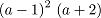
\includegraphics[keepaspectratio]{images/EMT4aljabar - Naila Khalidatus Salwa-124.png}}

\textgreater\$\&invert(A) with a=0

\[\begin{pmatrix}-\frac{1}{2} & \frac{1}{2} & \frac{1}{2} \\ \frac{1  }{2} & -\frac{1}{2} & \frac{1}{2} \\ \frac{1}{2} & \frac{1}{2} & -  \frac{1}{2} \\ \end{pmatrix}\]\textgreater A \&= {[}1,a;b,2{]}; \$A

\[\begin{pmatrix}1 & a \\ b & 2 \\ \end{pmatrix}\]Seperti semua variabel simbolik, matriks ini dapat digunakan dalam ekspresi simbolik lainnya.

\textgreater\$\&det(A-x*ident(2)), \$\&solve(\%,x)

\[\left[ x=\frac{3-\sqrt{4\,a\,b+1}}{2} , x=\frac{\sqrt{4\,a\,b+1}+3  }{2} \right] \]\pandocbounded{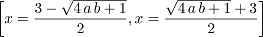
\includegraphics[keepaspectratio]{images/EMT4aljabar - Naila Khalidatus Salwa-128.png}}

Nilai eigen juga dapat dihitung secara otomatis. Hasilnya adalah sebuah vektor dengan dua vektor nilai eigen dan multiplisitas.

\textgreater\$\&eigenvalues({[}a,1;1,a{]})

\[\left[ \left[ a-1 , a+1 \right]  , \left[ 1 , 1 \right]  \right] \]Untuk mengekstrak vektor eigen tertentu memerlukan pengindeksan yang cermat.

\textgreater\$\&eigenvectors({[}a,1;1,a{]}), \&\%{[}2{]}{[}1{]}{[}1{]}

\[\left[ \left[ \left[ a-1 , a+1 \right]  , \left[ 1 , 1 \right]    \right]  , \left[ \left[ \left[ 1 , -1 \right]  \right]  , \left[   \left[ 1 , 1 \right]  \right]  \right]  \right] \]\\
{[}1, - 1{]}

Matriks simbolik dapat dievaluasi dalam Euler secara numerik sama seperti ekspresi simbolik lainnya.

\textgreater A(a=4,b=5)

\begin{verbatim}
            1             4 
            5             2 
\end{verbatim}

Dalam ekspresi simbolik, gunakan with.

\textgreater\$\&A with {[}a=4,b=5{]}

\[\begin{pmatrix}1 & 4 \\ 5 & 2 \\ \end{pmatrix}\]Akses ke deretan matriks simbolik berfungsi sama seperti matriks numerik.

\textgreater\$\&A{[}1{]}

\[\left[ 1 , a \right] \]Ekspresi simbolis dapat berisi tugas. Dan itu mengubah matriks A.

\textgreater\&A{[}1,1{]}:=t+1; \$\&A

\[\begin{pmatrix}t+1 & a \\ b & 2 \\ \end{pmatrix}\]Ada fungsi simbolik di Maxima untuk membuat vektor dan matriks. Untuk ini, lihat dokumentasi Maxima atau tutorial tentang Maxima di EMT.

\textgreater v \&= makelist(1/(i+j),i,1,3); \$v

\[\left[ \frac{1}{j+1} , \frac{1}{j+2} , \frac{1}{j+3} \right] \]\textgreater B \&:= {[}1,2;3,4{]}; \$B, \$\&invert(B)

\[\begin{pmatrix}-2 & 1 \\ \frac{3}{2} & -\frac{1}{2} \\   \end{pmatrix}\]\pandocbounded{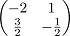
\includegraphics[keepaspectratio]{images/EMT4aljabar - Naila Khalidatus Salwa-136.png}}

Hasilnya dapat dievaluasi secara numerik dalam Euler. Untuk informasi lebih lanjut tentang Maxima, lihat pengenalan Maxima.

\textgreater\$\&invert(B)()

\begin{verbatim}
           -2             1 
          1.5          -0.5 
\end{verbatim}

Euler juga memiliki fungsi kuat xinv(), yang melakukan upaya lebih besar dan mendapatkan hasil yang lebih tepat.

Perhatikan, bahwa dengan \&:= matriks B telah didefinisikan sebagai simbolik dalam ekspresi simbolik dan numerik dalam ekspresi numerik. Jadi kita bisa menggunakannya di sini.

\textgreater longest B.xinv(B)

\begin{verbatim}
                      1                       0 
                      0                       1 
\end{verbatim}

Misalnya. nilai eigen dari A dapat dihitung secara numerik.

\textgreater A={[}1,2,3;4,5,6;7,8,9{]}; real(eigenvalues(A))

\begin{verbatim}
[16.1168,  -1.11684,  0]
\end{verbatim}

Atau secara simbolis. Lihat tutorial tentang Maxima untuk detailnya.

\textgreater\$\&eigenvalues((\textbf{A?}))

\[\left[ \left[ 3-\sqrt{10} , \sqrt{10}+3 , 1 \right]  , \left[ 1 , 1   , 1 \right]  \right] \]\# Contoh Lainnya

\textgreater A \&= {[}2,6,4;1,2,3;4,5,6{]}; \$A

\[\begin{pmatrix}2 & 6 & 4 \\ 1 & 2 & 3 \\ 4 & 5 & 6 \\ \end{pmatrix}\]\textgreater\$\&det(A)

\[18\]\textgreater B \&= makelist(1/(i+j),i,1,3); \$B

\[\left[ \frac{1}{j+1} , \frac{1}{j+2} , \frac{1}{j+3} \right] \]\textgreater A \&= {[}2,a;b,3{]}; \$A

\[\begin{pmatrix}2 & a \\ b & 3 \\ \end{pmatrix}\]\textgreater\$\&eigenvalues({[}b,2;4,a{]})

\[\left[ \left[ \frac{-\sqrt{b^2-2\,a\,b+a^2+32}+b+a}{2} , \frac{  \sqrt{b^2-2\,a\,b+a^2+32}+b+a}{2} \right]  , \left[ 1 , 1 \right]    \right] \]\# Nilai Numerik dalam Ekspresi simbolik

Ekspresi simbolis hanyalah string yang berisi ekspresi. Jika kita ingin mendefinisikan nilai untuk ekspresi simbolik dan ekspresi numerik, kita harus menggunakan ``\&:=''.

\textgreater A \&:= {[}1,pi;4,5{]}

\begin{verbatim}
            1       3.14159 
            4             5 
\end{verbatim}

Masih terdapat perbedaan antara bentuk numerik dan simbolik. Saat mentransfer matriks ke bentuk simbolik, pendekatan pecahan untuk real akan digunakan.

\textgreater\$\&A

\[\begin{pmatrix}t+1 & a \\ b & 2 \\ \end{pmatrix}\]Untuk menghindari hal ini, ada fungsi ``mxmset(variabel)''.

\textgreater mxmset(A); \$\&A

\[\begin{pmatrix}1 & 8 \\ 4 & 9 \\ \end{pmatrix}\]Maxima juga dapat menghitung dengan bilangan floating point, bahkan dengan floating point besar dengan 32 digit. Namun, evaluasinya jauh lebih lambat.

\textgreater\$\&bfloat(sqrt(2)), \$\&float(sqrt(2))

\[1.414213562373095\]\pandocbounded{
\includegraphics[keepaspectratio]{images/EMT4aljabar - Naila Khalidatus Salwa-146.png}}

Ketepatan angka floating point besar dapat diubah.

\textgreater\&fpprec:=100; \&bfloat(pi)

\begin{verbatim}
        3.14159265358979323846264338327950288419716939937510582097494\
4592307816406286208998628034825342117068b0
\end{verbatim}

Variabel numerik dapat digunakan dalam ekspresi simbolik apa pun menggunakan ``(\textbf{var?})''.

Perhatikan bahwa ini hanya diperlukan, jika variabel telah didefinisikan dengan ``:='' atau ``='' sebagai variabel numerik.

\textgreater B:={[}1,pi;3,4{]}; \$\&det((\textbf{B?}))

\[-5.424777960769379\]\# Contoh Lainnya

\textgreater A \&:= {[}1,8;4,9{]}

\begin{verbatim}
            1             8 
            4             9 
\end{verbatim}

\textgreater\$\&bfloat(sqrt(5))

\[2.2360679774997896964091736687313_B \times 10^{0}\]\textgreater\$\&float(sqrt(5))

\[2.23606797749979\]\textgreater mxmset(A); \$\&A

\[\begin{pmatrix}1 & 8 \\ 4 & 9 \\ \end{pmatrix}\]\textgreater\$\& det((\textbf{A?}))

\[-23\]\# Demo - Suku Bunga

Di bawah ini, kami menggunakan Euler Math Toolbox (EMT) untuk menghitung suku bunga. Kami melakukannya secara numerik dan simbolis untuk menunjukkan kepada Anda bagaimana Euler dapat digunakan untuk memecahkan masalah kehidupan nyata.

Asumsikan Anda memiliki modal awal sebesar 5.000 (katakanlah dalam dolar).

\textgreater K=5000

\begin{verbatim}
5000
\end{verbatim}

Sekarang kami mengasumsikan tingkat bunga 3\% per tahun. Mari kita tambahkan satu tarif sederhana dan hitung hasilnya.

\textgreater K*1.03

\begin{verbatim}
5150
\end{verbatim}

Euler juga akan memahami sintaks berikut.

\textgreater K+K*3\%

\begin{verbatim}
5150
\end{verbatim}

Namun lebih mudah menggunakan faktor tersebut.

\textgreater q=1+3\%, K*q

\begin{verbatim}
1.03
5150
\end{verbatim}

Selama 10 tahun, kita cukup mengalikan faktor-faktornya dan mendapatkan nilai akhir dengan tingkat bunga majemuk.

\textgreater K*q\^{}10

\begin{verbatim}
6719.58189672
\end{verbatim}

Untuk keperluan kita, kita dapat mengatur format menjadi 2 digit setelah titik desimal.

\textgreater format(12,2); K*q\^{}10

\begin{verbatim}
    6719.58 
\end{verbatim}

Mari kita cetak yang dibulatkan menjadi 2 digit dalam satu kalimat lengkap.

\textgreater{}``Starting from'' + K + ``\$ you get'' + round(K*q\^{}10,2) + ``\$.''

\begin{verbatim}
Starting from 5000$ you get 6719.58$.
\end{verbatim}

Bagaimana jika kita ingin mengetahui hasil antara dari tahun 1 sampai tahun ke 9? Untuk ini, bahasa matriks Euler sangat membantu. Anda tidak perlu menulis satu perulangan, tetapi cukup masuk

\textgreater K*q\^{}(0:10)

\begin{verbatim}
Real 1 x 11 matrix

    5000.00     5150.00     5304.50     5463.64     ...
\end{verbatim}

Bagaimana keajaiban ini terjadi? Pertama, ekspresi 0:10 mengembalikan vektor bilangan bulat.

\textgreater short 0:10

\begin{verbatim}
[0,  1,  2,  3,  4,  5,  6,  7,  8,  9,  10]
\end{verbatim}

Kemudian semua operator dan fungsi di Euler dapat diterapkan pada vektor elemen demi elemen. Jadi

\textgreater short q\^{}(0:10)

\begin{verbatim}
[1,  1.03,  1.0609,  1.0927,  1.1255,  1.1593,  1.1941,  1.2299,
1.2668,  1.3048,  1.3439]
\end{verbatim}

adalah vektor faktor q\^{}0 sampai q\^{}10. Ini dikalikan dengan K, dan kita mendapatkan vektor nilainya.

\textgreater VK=K*q\^{}(0:10);

Tentu saja, cara realistis untuk menghitung suku bunga ini adalah dengan membulatkan ke sen terdekat setiap tahunnya. Mari kita tambahkan fungsi untuk ini.

\textgreater function oneyear (K) := round(K*q,2)

Mari kita bandingkan kedua hasil tersebut, dengan dan tanpa pembulatan.

\textgreater longest oneyear(1234.57), longest 1234.57*q

\begin{verbatim}
                1314.82 
             1314.81705 
\end{verbatim}

Sekarang tidak ada rumus sederhana untuk tahun ke-n, dan kita harus mengulanginya selama bertahun-tahun. Euler memberikan banyak solusi untuk ini.

Cara termudah adalah fungsi iterate, yang mengulangi fungsi tertentu beberapa kali.

\textgreater VKr=iterate(``oneyear'',5000,10)

\begin{verbatim}
Real 1 x 11 matrix

    5000.00     5325.00     5671.13     6039.75     ...
\end{verbatim}

Kami dapat mencetaknya dengan cara yang ramah, menggunakan format kami dengan tempat desimal tetap.

\textgreater VKr'

\begin{verbatim}
    5000.00 
    5325.00 
    5671.13 
    6039.75 
    6432.33 
    6850.43 
    7295.71 
    7769.93 
    8274.98 
    8812.85 
    9385.69 
\end{verbatim}

Untuk mendapatkan elemen vektor tertentu, kami menggunakan indeks dalam tanda kurung siku.

\textgreater VKr{[}2{]}, VKr{[}1:3{]}

\begin{verbatim}
    5325.00 
    5000.00     5325.00     5671.13 
\end{verbatim}

Anehnya, kita juga bisa menggunakan vektor indeks. Ingatlah bahwa 1:3 menghasilkan vektor {[}1,2,3{]}.

Mari kita bandingkan elemen terakhir dari nilai yang dibulatkan dengan nilai penuh.

\textgreater VKr{[}-1{]}, VK{[}-1{]}

\begin{verbatim}
    9385.69 
  153925.27 
\end{verbatim}

Perbedaannya sangat kecil.

\chapter{Contoh Lainnya}\label{contoh-lainnya-16}

Akan digunakan formula berikut untuk menyelesaikan soal

\[S = P [\frac {(1+ \frac {r}{12})^{12\times t}-1}{\frac{r}{12}}]\]James menyetorkan \$250 setiap bulannya ke rekening pensiun dimulai

saat ia berusia 40 tahun. Jika investasi ini menghasilkan bunga 5\%

setiap tahunnya, berapa jumlah total tabungan pensiun James 27 tahun

kemudian?

Dari soal tersebut diketahui nilai

P = \$250

t = 27 tahun

r = 5\% = 0.05

\textgreater K=250

\begin{verbatim}
     250.00 
\end{verbatim}

\textgreater q=1+5\%, K*q

\begin{verbatim}
       1.05 
     262.50 
\end{verbatim}

\textgreater format(12,2); K*q\^{}(27)

\begin{verbatim}
     933.36 
\end{verbatim}

\textgreater short q\^{}(0:10)

\begin{verbatim}
[1,  1.05,  1.1025,  1.1576,  1.2155,  1.2763,  1.3401,  1.4071,
1.4775,  1.5513,  1.6289]
\end{verbatim}

\textgreater function oneyear (K) := round(K*q,2)

\textgreater longest oneyear(1234.57)

\begin{verbatim}
                 1296.3 
\end{verbatim}

\textgreater VKr=iterate(``oneyear'',250,27)

\begin{verbatim}
Real 1 x 28 matrix

     250.00      262.50      275.63      289.41     ...
\end{verbatim}

\textgreater VKr{[}27{]}

\begin{verbatim}
     888.95 
\end{verbatim}

\textgreater VKr{[}-1{]}, VK{[}-1{]}

\begin{verbatim}
     933.40 
  153925.27 
\end{verbatim}

Karena dengan cara sesuai contoh saya belum menemukan hasilnya, maka saya mnegerjakan sesuai formula yang terdapat di petunjuk

\textgreater P:=250; t:=27; r:=0.05; S= P*{[}((1+r/12)\^{}(12*t)-1)/(r/12){]}

\begin{verbatim}
  170797.30 
\end{verbatim}

Jadi, total uang tabungan pensiun James 27 tahun kemudian adalah \$170,797.30

Kayla menyetorkan \$100 ke rekening pensiun sejak ia berusia 25 tahun. Jika investasi ini menghasilkan bunga 4\% per tahun, dihitung secara bulanan, berapa banyak uang yang akan terkumpul di rekening Kayla ketika ia pensiun di usia 65 tahun?

Dari soal tersebut diketahui nilai

P = \$100

t = 65-25 = 40 tahun

r = 4\% = 0.04

\textgreater P:=100; t:=40; r:=0.04; S= P*{[}((1+r/12)\^{}(12*t)-1)/(r/12){]}

\begin{verbatim}
  118196.13 
\end{verbatim}

Jadi, banyak uang yang akan terkumpul di rekening Kayla ketika ia pensiun di usia 65 tahun adalah \$118,196.13

Sue dan Richard ingin membuat dana kuliah untuk putri mereka yang akan terkumpul sebesar \$120,000 pada akhir 18 tahun. Jika mereka mengandalkan suku bunga 3\%, dihitung setiap bulan, berapa banyak yang harus mereka setorkan setiap bulan untuk mencapai target tersebut?

Dari soal tersebut diketahui nilai

S = \$120,000

t = 18 tahun

r = 3\% = 0.03

\textgreater S=120000; t=18; r=0.03; P=S /{[}((1+r/12)\^{}(12*t)-1)/(r/12){]}

\begin{verbatim}
     419.67 
\end{verbatim}

Jadi, banyak uang yang harus mereka setorkan setiap bulan untuk mencapai target tersebut adalah \$419.67

Lamont ingin memiliki tabungan pensiun sebesar \$200,000 saat berusia 70 tahun. Jika ia mulai menyetorkan uang setiap bulan saat berusia 30 tahun dan mendapatkan bunga 4,5\% per tahun, berapa banyak uang yang harus dia simpan setiap bulan agar bisa mencapai target yang diinginkan?

Dari soal tersebut diketahui nilai

S = \$200,000

t = 70-30 = 40 tahun

r = 4.5\% = 0.045

\textgreater{} S=200000; t=40; r=0.045; P=S /{[}((1+r/12)\^{}(12*t)-1)/(r/12){]}

\begin{verbatim}
     149.13 
\end{verbatim}

Jadi, banyak uang yang harus dia simpan setiap bulan agar bisa mencapai target yang diinginkan adalah \$149.13

\chapter{Memecahkan Persamaan}\label{memecahkan-persamaan}

Sekarang kita mengambil fungsi yang lebih maju, yang menambahkan tingkat uang tertentu setiap tahunnya.

\textgreater function onepay (K) := K*q+R

Kita tidak perlu menentukan q atau R untuk definisi fungsi. Hanya jika kita menjalankan perintah, kita harus mendefinisikan nilai-nilai ini. Kami memilih R=200.

\textgreater R=200; iterate(``onepay'',5000,10)

\begin{verbatim}
Real 1 x 11 matrix

    5000.00     5450.00     5922.50     6418.63     ...
\end{verbatim}

Bagaimana jika kita menghapus jumlah yang sama setiap tahun?

\textgreater R=-200; iterate(``onepay'',5000,10)

\begin{verbatim}
Real 1 x 11 matrix

    5000.00     5050.00     5102.50     5157.63     ...
\end{verbatim}

Kami melihat uangnya berkurang. Jelasnya, jika kita hanya mendapat bunga sebesar 150 pada tahun pertama, namun menghapus 200, kita kehilangan uang setiap tahunnya.

Bagaimana kita dapat menentukan berapa tahun uang tersebut akan bertahan? Kita harus menulis satu lingkaran untuk ini. Cara termudah adalah dengan melakukan iterasi cukup lama.

\textgreater VKR=iterate(``onepay'',5000,50)

\begin{verbatim}
Real 1 x 51 matrix

    5000.00     5050.00     5102.50     5157.63     ...
\end{verbatim}

Dengan menggunakan bahasa matriks, kita dapat menentukan nilai negatif pertama dengan cara berikut.

\textgreater min(nonzeros(VKR\textless0))

\begin{verbatim}
       0.00 
\end{verbatim}

Alasannya adalah bukan nol (VKR\textless0) mengembalikan vektor indeks i, dengan VKR{[}i{]}\textless0, dan min menghitung indeks minimal.

Karena vektor selalu dimulai dengan indeks 1, maka jawabannya adalah 47 tahun.

Fungsi iterate() memiliki satu trik lagi. Ini dapat mengambil kondisi akhir sebagai argumen. Kemudian akan mengembalikan nilai dan jumlah iterasi.

\textgreater\{x,n\}=iterate(``onepay'',5000,till=``x\textless0''); x, n,

\begin{verbatim}
User interrupted!
onepay:
    useglobal; return K*q+R 
Try "trace errors" to inspect local variables after errors.
iterate:
    xn=f$(x,args());
\end{verbatim}

Mari kita coba menjawab pertanyaan yang lebih ambigu. Asumsikan kita mengetahui bahwa nilainya adalah 0 setelah 50 tahun. Berapa tingkat bunganya?

Ini adalah pertanyaan yang hanya bisa dijawab secara numerik. Di bawah ini, kita akan mendapatkan rumus yang diperlukan. Kemudian Anda akan melihat bahwa tidak ada rumus yang mudah untuk menentukan tingkat suku bunga. Namun untuk saat ini, kami menargetkan solusi numerik.

Langkah pertama adalah mendefinisikan fungsi yang melakukan iterasi sebanyak n kali. Kami menambahkan semua parameter ke fungsi ini.

\textgreater function f(K,R,P,n) := iterate(``x*(1+P/100)+R'',K,n;P,R){[}-1{]}

Iterasinya sama seperti di atas

\[x_{n+1} = x_n \cdot \left(1+ \frac{P}{100}\right) + R\]Namun kami tidak lagi menggunakan nilai global R dalam ekspresi kami. Fungsi seperti iterate() memiliki trik khusus di Euler. Anda dapat meneruskan nilai variabel dalam ekspresi sebagai parameter titik koma. Dalam hal ini P dan R.

Apalagi kami hanya tertarik pada nilai terakhir. Jadi kita ambil indeks {[}-1{]}.

Mari kita coba tes.

\textgreater f(5000,-200,3,47)

\begin{verbatim}
     -19.83 
\end{verbatim}

Sekarang kita bisa menyelesaikan masalah kita.

\textgreater solve(``f(5000,-200,x,50)'',3)

\begin{verbatim}
       3.15 
\end{verbatim}

Rutinitas penyelesaian menyelesaikan ekspresi=0 untuk variabel x. Jawabannya adalah 3,15\% per tahun. Kami mengambil nilai awal 3\% untuk algoritma. Fungsi solve() selalu membutuhkan nilai awal.

Kita dapat menggunakan fungsi yang sama untuk menyelesaikan pertanyaan berikut: Berapa banyak yang dapat kita keluarkan per tahun sehingga modal awal habis setelah 20 tahun dengan asumsi tingkat bunga 3\% per tahun.

\textgreater solve(``f(5000,x,3,20)'',-200)

Perhatikan bahwa Anda tidak dapat menyelesaikan jumlah tahun, karena fungsi kami mengasumsikan n sebagai nilai bilangan bulat.

\chapter{Contoh lainnya}\label{contoh-lainnya-17}

\textgreater function onepay (K) := K*q+R

\textgreater R=5\%; iterate(``onepay'',250,27)

\begin{verbatim}
Real 1 x 28 matrix

     250.00      262.55      275.73      289.56     ...
\end{verbatim}

\textgreater function f(K,R,P,n) := iterate(``x*(1+P/100)+R'',K,n;P,R){[}-1{]}

\textgreater f(250,-20,3,16)

\begin{verbatim}
      -1.96 
\end{verbatim}

\textgreater solve(``f(250,-20,x,16)'',3)

\begin{verbatim}
       3.06 
\end{verbatim}

\section{Solusi Simbolis Masalah Suku Bunga}\label{solusi-simbolis-masalah-suku-bunga}

Kita dapat menggunakan bagian simbolis dari Euler untuk mempelajari masalahnya. Pertama kita mendefinisikan fungsi onepay() kita secara simbolis.

\textgreater function op(K) \&= K*q+R; \$\&op(K)

\[R+q\,K\]Sekarang kita dapat mengulanginya.

\textgreater\$\&op(op(op(op(K)))), \$\&expand(\%)

\[q^3\,R+q^2\,R+q\,R+R+q^4\,K\]\pandocbounded{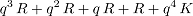
\includegraphics[keepaspectratio]{images/EMT4aljabar - Naila Khalidatus Salwa-156.png}}

Kami melihat sebuah pola. Setelah n periode yang kita miliki

\[K_n = q^n K + R (1+q+\ldots+q^{n-1}) = q^n K + \frac{q^n-1}{q-1} R\]Rumusnya adalah rumus jumlah geometri yang diketahui Maxima.

\textgreater\&sum(q\^{}k,k,0,n-1); \$\& \% = ev(\%,simpsum)

\[\sum_{k=0}^{n-1}{q^{k}}=\frac{q^{n}-1}{q-1}\]Ini agak rumit. Jumlahnya dievaluasi dengan tanda ``simpsum'' untuk menguranginya menjadi hasil bagi.

Mari kita membuat fungsi untuk ini.

\textgreater function fs(K,R,P,n) \&= (1+P/100)\^{}n*K + ((1+P/100)\^{}n-1)/(P/100)*R; \$\&fs(K,R,P,n)

\[\frac{100\,\left(\left(\frac{P}{100}+1\right)^{n}-1\right)\,R}{P}+K  \,\left(\frac{P}{100}+1\right)^{n}\]Fungsinya sama dengan fungsi f kita sebelumnya. Tapi ini lebih efektif.

\textgreater longest f(5000,-200,3,47), longest fs(5000,-200,3,47)

\begin{verbatim}
     -19.82504734650985 
     -19.82504734652684 
\end{verbatim}

Sekarang kita dapat menggunakannya untuk menanyakan waktu n.~Kapan modal kita habis? Perkiraan awal kami adalah 30 tahun.

\textgreater solve(``fs(5000,-330,3,x)'',30)

\begin{verbatim}
      20.51 
\end{verbatim}

Jawaban ini mengatakan akan menjadi negatif setelah 21 tahun.

Kita juga dapat menggunakan sisi simbolis Euler untuk menghitung rumus pembayaran.

Asumsikan kita mendapatkan pinjaman sebesar K, dan membayar n pembayaran sebesar R (dimulai setelah tahun pertama) meninggalkan sisa hutang sebesar Kn (pada saat pembayaran terakhir). Rumusnya jelas

\textgreater equ \&= fs(K,R,P,n)=Kn; \$\&equ

\[\frac{100\,\left(\left(\frac{P}{100}+1\right)^{n}-1\right)\,R}{P}+K  \,\left(\frac{P}{100}+1\right)^{n}={\it Kn}\]Biasanya rumus ini diberikan dalam bentuk

\[i = \frac{P}{100}\]\textgreater equ \&= (equ with P=100*i); \$\&equ

\[\frac{\left(\left(i+1\right)^{n}-1\right)\,R}{i}+\left(i+1\right)^{  n}\,K={\it Kn}\]Kita dapat menyelesaikan nilai R secara simbolis.

\textgreater\$\&solve(equ,R)

\[\left[ R=\frac{i\,{\it Kn}-i\,\left(i+1\right)^{n}\,K}{\left(i+1  \right)^{n}-1} \right] \]Seperti yang Anda lihat dari rumusnya, fungsi ini mengembalikan kesalahan floating point untuk i=0. Euler tetap merencanakannya.

Tentu saja, kami memiliki batasan berikut.

\textgreater\$\&limit(R(5000,0,x,10),x,0)

\[\lim_{x\rightarrow 0}{R\left(5000 , 0 , x , 10\right)}\]Yang jelas tanpa bunga kita harus membayar kembali 10 tarif 500.

Persamaan tersebut juga dapat diselesaikan untuk n.~Akan terlihat lebih bagus jika kita menerapkan beberapa penyederhanaan padanya.

\textgreater fn \&= solve(equ,n) \textbar{} ratsimp; \$\&fn

\[\left[ n=\frac{\log \left(\frac{R+i\,{\it Kn}}{R+i\,K}\right)}{  \log \left(i+1\right)} \right] \]\#\# Contoh lainnya

Akan digunakan formula berikut untuk menyelesaikan soal

\[M = P [\frac {\frac {r}{12}(1+ \frac {r}{12})^n}{(1+\frac{r}{12})^n -1}]\]Harga sebuah rumah adalah \$98,000 dengan uang muka \$16,000. Jika suku bunganya 6,5\% dan jangka waktu pinjaman 25 tahun, berapa besar angsuran bulanannya?

Dari soal diketahui nilai

P = \$98,000-\$16,000 = \$82,000

r = 6.5\% = 0.065

n = 25 tahun = 300 bulan

\textgreater P = 82000; r = 6.5\%; n = 300; P*{[}((r/12)*(1+ (r/12))\textsuperscript{n)/((1+(r/12))}n -1){]}

\begin{verbatim}
     553.67 
\end{verbatim}

Jadi, besar angsuran bulanannya adalah \$553.67

Harga sebuah rumah adalah \$124,000 dengan uang muka \$20,000. Jika suku bunganya 5,5\% dan jangka waktu peminjaman 30 tahun, berapa besar angsuran tiap bulannya?

Dari soal diketahui nilai

P = \$124,000 - \$20,000 = \$104,000

r = 5,5\%

n = 30 tahun = 360 bulan

\textgreater P = 104000; r = 5.5\%; n = 360; P*{[}((r/12)*(1+ (r/12))\textsuperscript{n)/((1+(r/12))}n -1){]}

\begin{verbatim}
     590.50 
\end{verbatim}

Jadi, besar angsuran bulanannya adalah \$590.50

Harga sebuah rumah adalah \$135,000 dengan uang muka \$18,000. Jika suku bunganya 7.75\% dan jangka waktu pinjaman 20 tahun, berapa besar angsuran bulanan yang harus dibayarkan?

Dari soal diketahui nilai

P = \$135,000 - \$18,000 = \$117,000

r = 7.75\%

N = 20 tahun = 240 bulan

\textgreater~P = 117000; r = 7.75\%; n = 240; P*{[}((r/12)*(1+ (r/12))\textsuperscript{n)/((1+(r/12))}n -1){]}

\begin{verbatim}
     853.79 
\end{verbatim}

Jadi, besar angsuran bulanannya adalah \$853.79

Harga sebuah rumah adalah \$151,000 dengan uang muka \$21,000. Jika bunganya 6,25\% dan jangka waktu pinjaman 25 tahun, berapa besar angsuran bulanannya?

Dari soal diketahui nilai

P = \$151,000 - \$21,000 = \$130,000

r = 6,25\%

n = 25 tahun = 300 bulan

\textgreater P = 130000; r = 6.25\%; n = 300; P*{[}((r/12)*(1+ (r/12))\textsuperscript{n)/((1+(r/12))}n -1){]}

\begin{verbatim}
     857.57 
\end{verbatim}

Jadi, besar angsuran bulanannya \$857.57

\textgreater//

\backmatter
\end{document}
